\documentclass[thesis.tex]{subfiles}

\begin{document}
\ifSubfilesClassLoaded{
    \setcounter{chapter}{7}
}

\chapter{Estimating transmission using mechanistic modelling} \label{SEIR}

In this chapter, I introduce mechanistic models for estimating the transmission of SARS-CoV-2, an alternative to the statistical approach in \cref{E-backcalc}.
Mechanistic models explicitly represent the infection process driving the spread of infectious disease, giving the model's state and parameters a biological and/or epidemiological interpretation.
% Of particular interest is that the basic reproduction number, $\R$, and the effective reproduction number, $R_e(t)$, which can both be calculated as functions of the model parameters; using \cref{E-backcalc}'s approach, additional modelling would be required to estimate these numbers.
In particular, this allows changes in transmission to be decomposed into the components of the model, \eg the number of contacts per day or the probability of transmission upon contact.
Furthermore, mechanistic models can be used for scenario-based modelling, which simulates the effect of interventions.
All of these properties make mechanistic models a useful tool for understanding and controlling infectious diseases.
However, they make stronger assumptions about the disease and population behaviour than statistical models.

The literature on mechanistic models is vast, having been developed for over a century; the model in \cref{SEIR:sec:SIR} was first formulated by \textcite{kermackContribution}.
In this chapter, I will discuss only the background relevant to the application.
For further details I recommend the tutorial paper \textcite{kretzschmarMathematical} or the textbook \textcite{keelingModeling}.

I start this chapter by introducing a generic framework for mechanistic modelling of infectious diseases (\cref{SEIR:sec:transmission-generic}).
% This framework is then applied to SARS-CoV-2 in \cref{SEIR:sec:transmission-application}.
It describes the \emph{transmission model}, corresponding to the infection process.
The transmission model needs to be linked to observations; in this chapter, that will be the CIS prevalence data.
The \emph{observation model}, introduced in \cref{SEIR:sec:observation}, is this link; it incorporates both the prevalence process and the observation process.
These two components form the mathematical model, which I then fit to data, requiring specification of an inference process, parameterisation, and priors (\cref{SEIR:sec:inference-implementation}).
This final formulation uses the transmission model from \textcite{birrellRealtime}, but a novel observation model.
I then use a simulation study to check this recovers the parameters successfully (\cref{SEIR:sec:sim-study}).
Having shown that the model can recover the parameters, I then apply it to the CIS data (\cref{SEIR:sec:application}).
Finally, I discuss the results, limitations, and extensions of this work (\cref{SEIR:sec:discussion}).

Notation in this chapter differs from the rest of this thesis.
I adopt conventions and notation familiar to the infectious disease modelling field, although the field's notation is not consistent between sources.
In particular, upper or lower case no longer signifies whether a variable is random or not, but this is clear from the context.

\section{Transmission models} \label{SEIR:sec:transmission-generic}

This section introduces the class of mechanistic transmission models known as \emph{compartmental} models.
Compartmental models are the most widely-used class of mechanistic infectious disease model.
A compartmental model is named because they place every member of the population under study into a compartment; each compartment representing a disease state (\eg susceptible).

A compartmental model consists of a state vector $\vec{x}(t)$ and a set of parameters $\vec{\theta}$~\autocite{birrellEvidence}.
The elements of $\vec{x}(t)$ are the latent proportion of the population (or number of individuals) in each compartment at time $t$.
The parameters $\vec{\theta}$ determine, along with the model structure, how the state vector changes over time.
Inference about $\vec{x}(t)$ and $\vec{\theta}$ is requires linking to data, $\vec{y}$, via an observation model, $p(\vec{y}(t) \mid \vec{x}, \vec{\theta})$ where $\vec{x}$ denotes conditioning on $\vec{x}(t)$ for all $t$~\autocite{birrellEvidence} (see \cref{SEIR:sec:observation}).
That is, the observation model specifies the likelihood of the data given the model state.

Compartmental models can be \emph{deterministic} or \emph{stochastic}.
Deterministic models are defined by the state vector $\vec{x}(t)$ being a deterministic function of the parameters $\vec{\theta}$ and the initial state $\vec{x}(0)$; equivalently, $\var(\vec{x}(t) \mid \vec{x}(0), \theta) = 0$~\autocite{birrellEvidence}.
% In most situations, the function is not analytically-tractable and requires numeric methods to solve.
%The transmission model corresponds to the infection process (see \cref{E-inc-prev:sec:infection-process}).
%There remains randomness in the observation model (described in \cref{SEIR:sec:observation}).

Stochastic models specify a probability distribution for the current state $p(\vec{x}(t) \mid \set{H}_t, \vec{\theta})$ where $\set{H}_t = \{ \vec{x}(t') \ssep t' < t \}$ is the epidemic's history and $\vec{\theta}$ are model parameters\todo{REF stochastic models}.
Stochastic models are most commonly specified in discrete time, using a Markov assumption.
A common simplification is to use discrete time and a Markov assumption; \ie $\vec{x}(t)$ is only defined for integer $t$ and $p(\vec{x}(t) \mid \set{H}_t, \vec{\theta}) = p(\vec{x}(t) \mid \vec{x}(t-1), \vec{\theta})$~\autocite{birrellEvidence}.
This relaxes the assumption of independent increments in the counting process formulation of the infection process (see \cref{E-inc-prev:sec:infection-process}).

Deterministic models are also known as \emph{mean-field} models because they represent the mean behaviour of a corresponding stochastic model.
When the number of infectious individuals is large, the law of large numbers implies that the mean-field behaviour is a good approximation of the fully stochastic model~\autocite[20]{diekmannMathematical}.
This is especially true when making noisy observations of the system, and that the stochastic differences between the stochastic and its mean are negligible compared to the observation noise.
A formalisation of this argument underpins the mean-field approximation of the prevalence process made in \cref{E-inc-prev:sec:observation-process}.

The remainder of this chapter uses only deterministic models.
This choice is appropriate for the the context this thesis considers because there were many individuals infectious with SARS-CoV-2 in this time period.
There are a wealth of introductory texts on stochastic models, I recommend \textcite[chapter 6]{keelingModeling} or \textcite{birrellEvidence}.


This chapter discusses deterministic models whose evolution is specified by a system of ODEs, $d\vec{x}/dt$.
In an ODE model, time is necessarily continuous.%, although discretised when solving (see \cref{SEIR:sec:inference-implementation}).
For concreteness, I use units of days throughout, although the model can use any unit of time.
The number or proportion of individuals in each compartment is also continuous; clearly, this is not true in reality but is a good approximation when the population is large.

In this section, I introduce the \emph{susceptible-infectious-recovered} (SIR) model and the extensions to it I require to appropriately model SARS-CoV-2.

% \Cref{SEIR:sec:SIR} introduces the \emph{susceptible-infectious-recovered} (SIR) model, the simplest compartmental model for a disease where individuals are immune to reinfection following their recovery.
% The name SIR derives from the structure of the model.
% In particular, the model divides the population into one of three states: susceptible, infectious, or recovered.

% This model has several assumptions which make it inappropriate to model SARS-CoV-2; therefore, in the remainder of this section I introduce standard extensions to the SIR model which relax these assumptions.
% First, in \cref{SEIR:sec:non-exponential}, I relax the assumption that the infectious period is exponentially-distributed to allow gamma distributions.
% Then, in \cref{SEIR:sec:SEIR}, I relax the assumption that individuals are infectious immediately after they are infected; it does this by extending the SIR model to the SEIR model with the additional E signifying an \emph{exposed} compartment.
% Finally, in \cref{SEIR:sec:structured-populations}, I include heterogeneity in the population, stratifying by important characteristic(s).
% Finally, \cref{SEIR:sec:time-varying-foi} relaxes the assumption of a constant transmission rate to allow for time-varying behavioural changes.


\subsection{The SIR model} \label{SEIR:sec:SIR}

\begin{figure}[h]
\makebox[\textwidth][c]{
\begin{tikzpicture}[
    node distance = 2.5cm,
    on grid,
    auto,
    ->,>=stealth',
    every state/.style={draw,rectangle},
    ]

    \node[state] (S) {$s$};
    \node[state, right=of S] (I) {$i$};
    \node[state, right=of I] (R) {$r$};

    \path (S) edge node {$\lambda(t)$} (I)
          (I) edge node {$\gamma$} (R);
\end{tikzpicture}
}
  \caption[The SIR model]{Schematic of the basic SIR model. Arrows are labelled with the rates at which individuals move between compartments.}
  \label{SEIR:fig:SIR}
\end{figure}

The simplest compartmental model for a disease which confers immunity is the (SIR) model\todo{ref for SIR being simplest} (depicted in \cref{SEIR:fig:SIR}).
The name SIR derives from the structure of the model.
In particular, the model divides the population (assumed closed, an assumption discussed later) into one of three compartments: susceptible, infectious, or recovered.
% The state of the system is the proportion of the population in each compartment.
In the SIR model, individuals are assumed to be homogeneous except for their disease state, \ie they are otherwise identical.

Individuals in the susceptible compartment are those that could be infected (they have no immunity).
The proportion of the population that is susceptible at time $t$ is $s(t)$.
Individuals in the infectious compartment can infect others, and eventually recover.
The proportion of the population that is infectious at time $t$ is $i(t)$.
Individuals in the recovered compartment are immune to the disease, and cannot be infected again.
The proportion of the population that have recovered by time $t$ is $r(t)$.
The model's state is $\vec{x}(t) = (s(t), i(t), r(t))^T$.

The SIR model is described by the following system of ODEs~\autocite[19]{keelingModeling}:
\begin{align}
\frac{ds(t)}{dt} &= -\lambda(t) s(t) \\
\frac{di(t)}{dt} &= \lambda(t) s(t) - \gamma i(t) \\
\frac{dr(t)}{dt} &= \gamma i(t)
\end{align}
where $\lambda(t) = \beta i(t)$, is the \emph{force of infection}: the risk of infection for a susceptible individual at time $t$~\autocite[17]{keelingModeling}.
The dynamics of the model are described by the parameters $\vec{\theta} = (\beta, \gamma)^T$.
$\beta$ is the transmission rate, absorbing several terms as described below.
$\gamma$ is the recovery rate, or the rate that infectious individuals that recover per day; hence, $1/\gamma$ is the mean infectious period~\autocite[367]{keelingModeling}.
These parameters are assumed to be constant.

% The term $\beta s(t)i(t)$ is the rate at which susceptible individuals (as a proportion of the total population size) are infected~\autocite[18]{keelingModeling}.
% Susceptible individuals move from the $s(t)$ to $i(t)$ when they are infected.
The expression for the force of infection, $\lambda(t)$ can be arrived at by considering a single infectious individual~\autocite[214]{kretzschmarMathematical}.
Assume this individual, on average, comes into contact with other individuals in the population at a rate of $\kappa$.
Further, assume the population is \emph{well-mixed}, meaning that each contact is with an individual chosen uniformly at random from the population; this is implied by assuming a homogeneous population.
For such a randomly selected individual, the probability that they are susceptible is $s(t)$.
% Each of the infectious individual's contacts is therefore with a susceptible individual with probability $s(t)$, by the well-mixed assumption.
Therefore, in expectation, the infectious individual makes contact with susceptible individuals at a rate of $\kappa s(t)$ per day.
Assume that there is a constant probability of transmission upon contact between an infectious and susceptible individual, $q$.
Combined with the above, the expected rate of infections caused by this infectious individual is $\kappa s(t) q$ per day.
The two constant terms here (number of contacts and probability of transmission) are absorbed into the transmission rate, $\beta = \kappa q$.
Therefore, the rate of new infections generated by a single infectious individual is $\beta s(t)$ per day.
Multiplying by the number of infectious individuals and dividing by the population size gives the rate per day at which susceptible individuals are infected as a proportion of the population, $\beta s(t) i(t) = \lambda(t) s(t)$.

% The term $\gamma i(t)$, the rate at which infectious individuals (as a proportion of the total population size) recover, follows directly from the definitions of $\gamma$ and $i(t)$.

A few properties and assumptions of the SIR model are worth noting.
\begin{itemize}
    \item For any short period of time when $s(t)$ is approximately constant, the solution to the system of ODEs includes exponential growth in the number of infectious individuals: $i(t) = i_0 e^{\psi t}$ for some constants $i_0$ and $\psi$~\autocite[section 1.2]{diekmannMathematical}.
    A notable example is the early part of an epidemic when $s(t) \approx 1$.
    This is the phase of initial exponential growth of an epidemic, which produces the characteristic early epidemic curves.
    It is in this phase that the basic reproduction number provides a good approximation of the epidemic dynamics.
    \item The basic reproduction number for the SIR model is $\R = \beta / \gamma$~\autocite[20]{keelingModeling}.
    Intuitively, this can be thought of as the average number of infections caused by an infectious individual per day, $\beta$, multiplied by the average number of days for which they are infectious, $1/\gamma$.
    \item The effective reproduction number for this model is $R_e(t) = \beta / \gamma s(t) = \R s(t)$~\autocite{pellisEstimation}.
    $1-s(t)$ is the fraction of infections that are avoided because of the presence of immune individuals in the population.
    \item The population is assumed to be closed.
    This assumption implies several attributes.
    First, the total population size is constant.
    Second, only a negligble number of infections are imported from outside the population.
    Third, births and deaths of individuals are negligble over the length of time considered; simple extensions allow including them~\autocites[26]{keelingModeling}[214]{kretzschmarMathematical}.
    \item There is no analytical solution to the system of ODEs: numerical methods are required to solve the system~\autocite[25]{keelingModeling}.
    \item As notes previously, the parameters $\vec{\theta}$ and the intial state of the system, $\vec{x}(0)$ is required to solve the system.
    \item Immunity is assumed to last until the end of the  period considered ~\autocite[61]{andersonInfectious}.
    In many contexts, including here, this assumption is justified because the period is shorter than the length of immunity conferred~\autocite{milneImmunity}.
    For longer time periods, waning immunity can be incorporated by allowing individuals to move from the recovered compartment back to the susceptible compartment~\autocite[40]{keelingModeling}.
\end{itemize}


\subsection{Non-exponential waiting times} \label{SEIR:sec:non-exponential}
\begin{figure}[h]
\makebox[\textwidth][c]{
\begin{tikzpicture}[
    node distance = 2.5cm,
    on grid,
    auto,
    ->,>=stealth',
    every state/.style={draw,rectangle},
    ]

    \node[state] (S) {$s$};
    \node[state, right=of S] (I1) {$i_1$};
    \node[state, right=of I1] (I2) {$i_2$};
    \node[state, right=of I2, draw=none] (I3) {$\cdots$};
    \node[state, right=of I3] (I4) {$i_n$};
    \node[state, right=of I4] (R) {$r$};

    \path (S) edge node {$\beta i$} (I1)
          (I1) edge node {$n\gamma$} (I2)
          (I2) edge node {$n\gamma$} (I3)
          (I3) edge node {$n\gamma$} (I4)
          (I4) edge node {$n\gamma$} (R);
\end{tikzpicture}
}
  \caption[The SIR model with non-exponential infectious period]{Schematic of the SIR model with non-exponential infectious period. The infectious period is modified by having multiple I states.}
  \label{SEIR:fig:SIR-gamma}
\end{figure}

The basic SIR model implies that the distribution of the time spent in the infectious compartment is exponential~\autocite[96]{keelingModeling}.
This is an unrealistic assumption for most diseases and would lead to underestimating of the reproduction number~\autocites{lloydRealistic}{wearingAppropriate}.
A standard extension to the SIR model is to allow the infectious period to follow a gamma distribution~\autocite[94]{keelingModeling}.
This is done by adding multiple infectious compartments, shown in \cref{SEIR:fig:SIR-gamma}.
The system can now be written as follows:
\begin{align}
\frac{ds(t)}{dt} &= -\lambda(t) s(t)\\
\frac{di_1(t)}{dt} &= \lambda(t) s(t) - n\gamma i_1(t) \\
\frac{di_2(t)}{dt} &= n\gamma i_1(t) - n \gamma i_2(t) \\
&\vdots \nonumber \\
\frac{di_n(t)}{dt} &= n\gamma i_{n-1}(t) - n \gamma i_n(t) \\
\frac{dr(t)}{dt} &= n\gamma i_n(t)
\end{align}
where $n$ is the number of infectious compartments, and redefining $\lambda(t) = \beta \sum_{j=1}^n i_j(t)$.
In this model the infectious period is distributed $\GamDist(n, n\gamma)$, a realistic model for a variety of diseases~\autocite{wearingAppropriate}.
This parameterisation is chosen to give $1/\gamma$ as the mean infectious period (further details on the Gamma distribution are in \cref{E-distributions}).
A gamma distribution with the first parameter equal to 1 is an exponential distribution, in which case this model collapses to the basic SIR model in \cref{SEIR:sec:SIR}.
As $n$ increases, the between-individual variability in infectious period length reduces, tending to a constant as $n \to \infty$~\autocite{lloydRealistic}.

The new compartments are biologically identical, without an interpretation differentiating the compartments.
They should be considered as a mathematical trick so that the ODE system produces a gamma distribution rather than an interpretable quantity.

% (it is slightly unclear what it means for a variable to have a distribution in a deterministic model, the clearest explanation is that this is the distribution which the ).

The reproduction number in terms of the parameters is unchanged by this extension, \ie $\R = \beta / \gamma$.

\subsection{The SEIR model} \label{SEIR:sec:SEIR}

\begin{figure}[h]
\makebox[\textwidth][c]{
\begin{tikzpicture}[
    node distance = 2cm,
    on grid,
    auto,
    ->,>=stealth',
    every state/.style={draw,rectangle},
    % remember picture, overlay
    ]

    \node[state, xshift=-2cm] (S) {$s$};
    \node[state, right=of S] (E1) {$e_1$};
    \node[state, right=of E1] (E2) {$e_2$};
    \node[state, right=of E2, draw=none] (E3) {$\cdots$};
    \node[state, right=of E3] (E4) {$e_m$};
    % \node[state, right=of E4] (I1) {$i_1$};
    \node[state, below=of E1] (I1) {$i_1$};
    \node[state, right=of I1] (I2) {$i_2$};
    \node[state, right=of I2, draw=none] (I3) {$\cdots$};
    \node[state, right=of I3] (I4) {$i_n$};
    \node[state, right=of I4] (R) {$r$};

    \path (S) edge node {$\beta i$} (E1)
          (E1) edge node {$m\sigma$} (E2)
          (E2) edge node {$m\sigma$} (E3)
          (E3) edge node {$m\sigma$} (E4)
          (I1) edge node {$n\gamma$} (I2)
          (I2) edge node {$n\gamma$} (I3)
          (I3) edge node {$n\gamma$} (I4)
          (I4) edge node {$n\gamma$} (R);
    \draw[->] (E4.east) -- ++(1,0) |- ([yshift=-1cm]E4.east) node [near start, right] {$m\sigma$} -|  (I1.north);
\end{tikzpicture}
}
  \caption[The SEIR model]{Schematic of the SEIR model.}
  \label{SEIR:fig:SEIR}
\end{figure}

The SIR model assumes that individuals are immediately infectious upon infection.
This is unrealistic for most diseases, as there is a period between an individual being infected and them being infectious, known as the \emph{latent period}.
\todo{I will probably end up defining the latent period in the intro, so should just ref that}
Ignoring the latent period will again overestimate the reproduction number~\autocite{wearingAppropriate}.

The SIR model can be extended to include a latent period by adding a latent compartment~\autocite[41]{keelingModeling}, also known as an \emph{exposed} compartment.
This forms the susceptible-exposed-infectious-recovered (SEIR) model, shown in \cref{SEIR:fig:SEIR}.

Similar to the infectious period, the latent period can be modelled as a gamma distribution by adding multiple latent compartments.
\begin{align}
\frac{ds}{dt} &= -\beta si \\
\frac{de_1}{dt} &= \beta si - m\sigma e_1 \\
\frac{de_2}{dt} &= m\sigma e_1 - m \sigma e_2 \\
&\vdots \nonumber \\
\frac{de_m}{dt} &= m\sigma e_{m-1} - m \sigma e_m \\
\frac{di_1}{dt} &= m\sigma e_m - n\gamma i_1 \\
\frac{di_2}{dt} &= n\gamma i_1 - n \gamma i_2 \\
&\vdots \nonumber \\
\frac{di_n}{dt} &= n\gamma i_{n-1} - n \gamma i_n \\
\frac{dr}{dt} &= n\gamma i_n
\end{align}
where $m$ is the number of latent compartments and $1/\sigma$ is the mean duration of the latent period.
The latent period is distributed $\GamDist(m, m\sigma)$ and the infectious period is still distributed $\GamDist(n, n\gamma)$.

The reproduction number in terms of the parameters is unchanged by this extension, \ie $\R = \beta / \gamma$, however, the growth rate in the exponential phase will be slower than before~\autocite[41]{keelingModeling}.

\subsection{Structured populations} \label{SEIR:sec:structured-populations}

To relax the assumption of a homogeneous population, the population can be stratified.
If the strata have differing transmission patterns, this can change the dynamics of the epidemic.
The different patterns could be due to behavioural factors (\eg high-numbers of sexual partners in a sexually-transmitted disease~\autocite[69]{keelingModeling} or younger age groups making many more contacts for respiratory diseases~\autocite[176]{andersonInfectious}), or biological factors such as genetics~\autocite[208]{andersonInfectious}.
I will assume that the disease progression (\ie length of the exposed and infectious periods) is the same for all strata, although this assumption can be relaxed.
Stratification requires two major  model changes: extension of the state vector and a description of the between-strata interactions.

The state vector is now a vector of vectors, one for each of the compartments.
I denote the set of strata, as $\set{A}$, with the set's size as $A$.
For example, in the basic SIR model, $\vec{x}(t) = (\vec{s}(t), \vec{i}(t), \vec{r}(t))^T$.
Element $a \in \set{A}$ of each vector is the proportion of strata $a$ in that compartment.
For example, $\vec{s}(t) = (s_1(t), \dots, s_A(t))^T$ where $s_a(t)$ is the proportion of the $a$th strata that are susceptible at time $t$.
Hence, $N_a s_a(t)$ is the number of susceptible people in stratum $a$, where $N_a$ is the number of individuals in stratum $a$.
These vectors replace the scalars in the previous equations.
Other, equivalent formulations of this model exist within the literature.
For example defining $s_a$ as the proportion of the total population that are both in strata $a$ and susceptible or parameterised using numbers of individuals~\autocite[57]{keelingModeling}, rather than as the proportion of strata $a$ as I have done here.

The interactions between strata are included by replacing the scalar $\beta$ with a \emph{Who Acquires Infection From Whom} (WAIFW) matrix, $\matr{\beta}$~\autocite[58]{keelingModeling}.
The force of infection is now a vector, defined as $\vec\lambda(t) = \matr{\beta} \sum_{j=1}^n \vec{i_j}(t)$.
Their interpretation can be arrived at by considering a single infectious individual in strata $a'$, analogous to the single stratum case.
Assume any such individual comes into contact with individuals in strata $a$ at a rate $\kappa_{aa'}$ per day.
% Further, assume that each contact is with an individual chosen uniformly at random from within the strata.
% For such a randomly selected individual, the probability that they are susceptible is $s_a(t)$.
% Each of the infectious individual's contacts is therefore with a susceptible individual with probability $s(t)$, by the well-mixed assumption.
Following the same argument as in \cref{SEIR:sec:SIR} finds that, in expectation, the infectious individual makes contact with susceptible individuals in stratum $a$ at a rate of $\kappa_{aa'} s_a(t)$ per day.
Now assume that there is a constant probability of transmission upon contact between an infectious individual in strata $a'$ and susceptible in strata $a$ individual, $q_{aa'}$.
Therefore, the expected rate of infections in strata $a$ caused by this infectious individual is $\kappa_{aa'} s_a(t) q_{aa'}$ per day.
Multiplying by the number of infectious individuals in strata $a'$, $N_{a'} i_{a'}(t)$, gives $\kappa_{aa'} q_{aa'} s_a(t) N_{a'} i_{a'}(t)$ where $i_{a'}(t) = \sum_{j=1}^n i_{j,a'}$ is the total proportion of stratum $a'$ that is infectious, regardless of which compartment they are in.
The constant terms here are absorbed into the WAIFW matrix, hence $\beta_{aa'} = \kappa_{aa'} q_{aa'} N_{a'}$~\autocite[section 9.2]{diekmannMathematical}.
The total force of infection on strata $a$ from all strata is, therefore, $\lambda_a(t) = \sum_{a' \in \set{A}} \beta_{aa'} i_{a'}(t)$.
Equivalently, $\vec\lambda(t) = \matr{\beta} \sum_{j=1}^n \vec{i_j}(t)$.
If all $\beta_{aa'}$ are equal, then the model is equivalent to the homogeneous model (\ie without any structure).
The rate at which individuals move between the susceptible and exposed compartments is now $\vec{s}(t) \circ \vec\lambda(t)$, where $\circ$ denotes element-wise multiplication.

In practical situations, estimating all the $\beta_{aa'}$ parameters is infeasible, so some assumptions must be made to reduce the number of parameters~\autocite[176]{andersonInfectious}.
It is infeasible because the progression of the epidemic depends on $\vec{\lambda}(t)$, which has dimension $A$, while $\matr{\beta}$ has dimension $A^2$.
Common assumptions include assuming symmetry, \ie $\beta_{aa'} = \beta_{a'a}$, or that the direction of transmission is irrelevant, \ie $\beta_{aa'} = \beta_{a} \beta_{a'}$.
% Alternatively, as in the scalar case, it may be easier to iden $\beta_{aa'}$ can be decomposed into the contact rate between strata $a$ and $a'$, $\kappa_{aa'}$ and the probability of transmission upon contact, $q_{aa'}$, and then assumptions made about the components.
The choice of assumptions depends on the context, including the disease being studied and the data available.

Reproduction numbers in models with structured populations need to consider the distribution of infections across the strata.
The WAIFM allows calculation of the number of secondary infections generated by a single infection in the $a$th strata,  this follows directly from its definition as $\frac{1}{\gamma} \sum_{a' \in \set{A}} \beta_{aa'}$. 
However, how to average these contributions to calculate the basic reproduction number is not obvious.
The standard solution to this was proposed by \textcite{diekmannDefinition} (see \textcite[chapter 7]{diekmannMathematical} for a more gentle, but still rigorous, explanation).
First, they show that the distribution of infections across the strata during the initial period of exponential growth (when $\vec{s} \approx \vec{1}$) relies only on $\matr{\beta}$.
This distribution is proportional to the \emph{dominant eigenvector} (the eigenvector corresponding to the largest eigenvalue) of $\matr{\beta}$.
Denote by $D(\matr{\beta})$ the \emph{dominant eigenvalue} (the largest eigenvalue).
The basic reproduction number is then defined as $\R = D(\matr{\beta}) / \gamma$.
This $\R$ keeps the same interpretation as in the homogeneous case, \ie the average number of secondary infections caused by a single infection in a fully susceptible population, where the average is taken over the distribution implied by the dominant eigenvector.
The important threshold that exponential growth occurs iff $\R > 1$ remains.

Age-based contact patterns are important for the transmission dynamics of respiratory diseases~\autocites{birrellBayesian}{jacksonEffects}.
Respiratory diseases can be spread by conversational contacts, which show very clear age patterns (see \cref{SEIR:fig:age-contacts}).
In particular, the contacts are \emph{associative} (contacts are more likely between individuals of similar ages) and younger age groups have more contacts; this will tend to concentrate the epidemic in these younger age groups~\autocite[67]{keelingModeling}.
\begin{figure}
  \centering 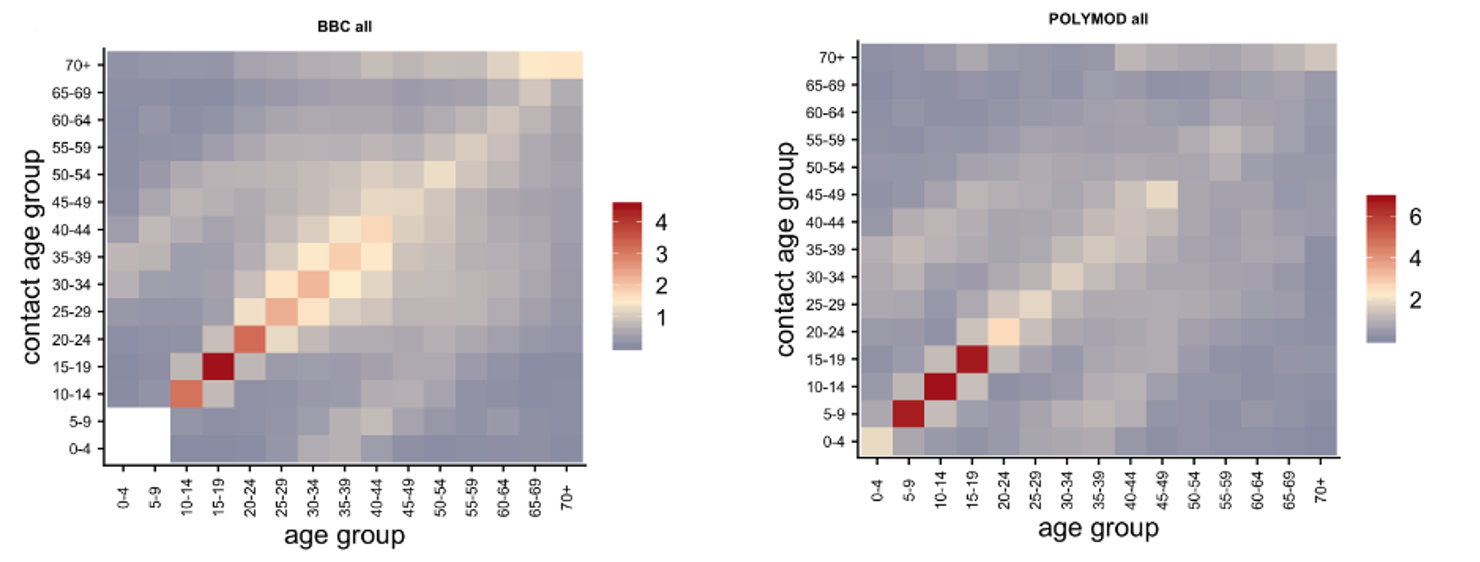
\includegraphics[width=\textwidth]{SEIR/contact_matrices}
  \caption[Age-based contact matrices]{Number of contacts reported between age groups in two contact surveys: (A) number of contacts reported in the POLYMOD survey~\autocite{mossongSocial}; (B) number of contacts reported in the BBC Pandemic survey~\autocite{klepacContacts}, which only collected data on those aged over 12. A clear diagonal, showing associative mixing is visible, and children have more contacts. Parallel diagonals off the main diagonal show mixing between parents and their children. Figure adapted from \textcite{klepacContacts}.}
  \label{SEIR:fig:age-contacts}
\end{figure}

\section{Observation model} \label{SEIR:sec:observation}

A variety of different approaches can be taken to link a transmission model to observations.
The method to do so is known as the observation model.
The formulation of this model is heavily dependent on the data available.
This means that there is a wide variety of models used.
Therefore, this section  explains the model I propose for fitting to the CIS prevalence data.

% Here, I extend the system of ODEs to include compartments representing PCR positive individuals.
% The proportion of PCR positive individuals in each strata is then linked to the CIS using a Beta-Binomial likelihood, with the modelled proportion that are PCR positive as the mean of the Beta distribution.
One approach would be to convolve the incidence based on the transmission model with the PCR duration distribution.
Here incidence is calculated from the ODE solution and then related to the data as explained in \cref{E-inc-prev}.
However, this approach is computationally expensive because of the need to calculate the convolution in \cref{E-inc-prev:eq:EPt }.

A much more efficient option is to approximate this convolution by adding compartments to the ODEs.
This approach also allows the infected, pre-positive compartment, which I denote $p_0$, to be represented.
$p_0$ increases at the same rate as individuals flow into $e_1$.
These individuals then transition into a set of compartment with their transition rates chosen to match the duration of positivity estimates in \cref{E-imperf-test}, $p_1, \dots, p_l$.
These compartments do not have a biological interpretation, unlike the other compartments in the system, but are purely a mathematical tool so that the time spent in these compartments matches the duration distribution.
This is the same idea behind having multiple exposed or latent compartments (introduced in \cref{SEIR:sec:non-exponential}).

Deciding $l$ and the length of time each individual spends in each compartment is the most challenging part of formulating the observation model.
The class of distributions which can be represented as a series of compartments are known as \emph{phase-type} distributions.
Discussions of general phase-type distributions are beyond the scope of this thesis; a review in a biological context can be found in \textcite{hobolthPhasetype}.
I will restrict myself to the subset of phase-type distributions defined by \textcite{osogamiClosed} as Erlang-Coxian (EC) distributions.
EC distributions are convenient because they are flexible enough to approximate almost any distribution, and the parameters of the approximation are given by closed-form functions of the distribution's moments.

% Formally, a phase-type distribution as the distribution of \emph{absorption time} in a \emph{continuous-time Markov process} with a single absorbing state~\autocite{hobolthPhasetype}.
% Given a probability distribution over starting states, a rate at which 
% The process can be defined by its size, $l$, a $l \times l$ \emph{transition matrix}, $\matr{M} \in \reals^{l \times l}$, an \emph{exit rate} vector, $\vec{\alpha}$ 
% The process's state at time $t$, $W_t$, is a scalar $W_t \in \{ 1, \dots, l+1 \}$.
% Its transition matrix is defined, for $j \neq k$, as $\prob(W_{t+\delta t} = k \mid ) = M_{jk} \delta t$ for small, positive $\delta t$.
% The diagonal is defined as $M_{jj} = - \sum_{k \neq j} M_{jk}$ so that the matrix $\matr{M}$ has row sums 0.
% The state $l+1$ is an absorbing state, that is $\prob(W_{t+t'} = l+1 \mid W_t = l_1) = 1$ for any non-negative $t'$ (once the process enters it, it cannot leave).
% The exit rate gives the transition rates into the absorbing state: $\prob(W_{t+\delta t} = l + 1 \mid W_t = j) = \alpha_j \delta t$ for small $\delta t$.
% The process's absorption time is when it first arrives at the absorbing state, $\tau = \inf \{ t \ssep W_t = l+1 \}$.
% That is, $P$ is a phase-type distribution if it can be represented as a process 
% They are additions of arbitrary exponential distributions, and can (if there is no limit on the number of compartments used) represent any distribution.
% \todo{check/cite these claims}
% I use the method of \textcite{osogamiClosed} to determine $l$ and the transition rates between the compartments.

% A $l$-phase EC distribution is the sum of a $(l-2)$-phase gamma distribution and a two-phase acyclic, arbitrary phase-type distribution.
An EC distribution $P$ can be defined as the sum of three random variables: $K$, $X_1$, and $X_2$.
It is shown schematically in \cref{SEIR:fig:EC}.
Here, $K \dist \GamDist(l-2, \kappa_Y)$, $X_1 \dist \Exponential(\kappa_{X1})$ and $X_2$ is a mixture distribution taking the value 0 with probability $1-p_x$ or otherwise (\ie with probability $p_x$) distributed $\Exponential(\kappa_{X2})$.
% The time between entering the 1st state and the $l+1$th state, the absorbing state, is the duration.
Gamma distributions with integer first parameters (as $K$ has) are also known as Erlang distributions.
The distribution $X_1 + X_2$ is a special case of the Coxian distribution.
Hence, the overall distribution is known as a Erlang-Coxian distribution.

\begin{figure}
\makebox[\textwidth][c]{
\begin{tikzpicture}[
    node distance = 2.5cm,
    on grid,
    auto,
    ->,>=stealth',
    every state/.style={draw,rectangle},
    ]

    \node[state] (1) {1};
    \node[state, right of=1] (2) {2};
    \node[state, right of=2, draw=none] (dots) {$\dots$};
    \node[state, right of=dots] (lm2) {$l-2$};
    \node[state, right of=lm2] (lm1) {$l-1$};
    \node[state, right of=lm1] (l) {$l$};
    \node[state, right of=l, align=center] (absorbing) {absorbing\\state};

    \path (1) edge node {$\kappa_Y$} (2)
          (2) edge node {$\kappa_Y$} (dots)
          (dots) edge node {$\kappa_Y$} (lm2)
          (lm2) edge node {$\kappa_Y$} (lm1)
          (lm1) edge node {$p_x \kappa_{X1}$} (l)
                edge [out=-45,in=-135] node[below] {$(1 - p_x) \kappa_{X1}$} (absorbing)
          (l) edge node {$\kappa_{X2}$} (absorbing);
\end{tikzpicture}
}
\caption[A $l$ phase EC distribution.]{Representation of an EC distribution as a series of compartments. The distribution is the time from entering state 1 and entering the absorbing state. The time between entering state 1 and state $l-2$ is distributed $K \dist \GamDist(l-2, \kappa_Y)$, also known as an Erlang distribution. The time between entering state $l-2$ and the absorbing state has a Coxian distribution (see the main text for details).}
\label{SEIR:fig:EC}
\end{figure}

\Textcite{osogamiClosed} define $P$ as well-matching an arbitrary distribution $G$ if $P$ and $G$ have the same first three moments.
They then prove that EC distributions have the following properties:
\begin{itemize}
    \item If there exists a phase-type distribution $P'$ that well-matches $G$ then there exists an EC distribution $P$ that well-matches $G$.
    \item The parameters of $P$ are available in closed form, and the expression for these is derived.
    \item The number of phases used by the $P$ calculated by these expressions is at most one more than the minimum across all phase-type distributions that well-match $G$.
\end{itemize}

A total of five parameters are required to specify a $l$-phase EC distribution.
\begin{itemize}
    \item $l$, the number of phases.
    \item $\kappa_Y$, the rate parameter of the Erlang distribution.
    \item $\kappa_{X1}$, the rate parameter of the first state after the Erlang distribution.
    \item $\kappa_{X2}$, the rate parameter of the second state after the Erlang distribution.
    \item $p_x$, the probability of moving from the end state of the Erlang distribution to the second (as opposed to directly to the absorbing state).
\end{itemize}

I use the mapfit package~\autocite{mapfit} to compute $P$ for the posterior mean of the distribution estimated in \cref{E-imperf-test}.
This is the same duration distribution used in \cref{E-backcalc}.
The parameter estimates are in \cref{SEIR:table:ec-params}.
\begin{table}
    \centering
    \begin{tabular}{c c c c c}
        $l$ & $\kappa_Y$ & $\kappa_{X1}$ & $\kappa_{X2}$ & $p_x$ \\
        3 & 0.0820 & 0.126 & 0.0223 & 0.00973  \\
    \end{tabular}
    \caption{Parameter estimates for the EC distribution approximating the posterior mean of the duration distribution estimated in \cref{E-imperf-test}.}
    \label{SEIR:table:ec-params}
\end{table}
% end table of ec params

The modelled proportion of individuals that are PCR positive in the can then be linked to the data using a Beta-Binomial likelihood (see\todo{ref section on clustering} for the issues with using a binomial likelihood).
If on each day $t$, each strata $i$ is observed to have $y_{it}$ positives out of $n_{it}$ tests, then the likelihood is:
\begin{align}
    \prod_{a,t} \BB (y_{at} \mid n_{at}, \sum_{k=1}^l \bar{p}_{kat}, \rho)
    \label{SEIR:eq:likelihood}
\end{align}
where $\bar{p}_{kat} = \int_{t}^{t+1} p_{ka}(s) ds$ is the mean occupancy in compartment $p_k$ and strata $a$ over day $t$ and $\rho$ is a nuisance parameter controlling the overdispersion of the beta-binomial distribution.
In this parameterisation (detailed in \cref{E-distributions}) at $\rho=0$ the beta-binomial coincides with the binomial distribution and as $\rho \to \infty$, the distribution tends towards the uniform distribution on $[0, 1]$~\autocite{hughesUsing}.

\section{Implementation} \label{SEIR:sec:inference-implementation}

\todo[inline]{Redo intro paragraph to "implementation" section}

The ultimate aim of this chapter is to infer the transmission dynamics from the CIS prevalence data.
This section considers the practicalities of achieving this aim via mechanistic models.

\subsection{WAIFW matrix}

A parsimonious model is needed to parameterise the WAIFW matrix (see \cref{SEIR:sec:structured-populations}).
I use the following age-based strata, which align closely with the age groupings previously used for analysis of the CIS data~\autocites[e.g.:][]{houseInferring}{walkerTracking}.
\todo{Contrast with age groupings used in previous chapter}
\begin{enumerate}
    \item $[0, 11)$: children of pre-school and primary school age.
    \item $[11, 16)$: children of compulsory secondary-school age.
    \item $[16, 25)$: adolescents and young adults who may remain in formal education.
    \item $[25, 50)$: younger working age adults.
    \item $[50, 70)$: older working age adults.
    \item $[70, \infty)$: elderly.
\end{enumerate}

I follow the WAIFW matrix parameterisation of \textcite{birrellRealtime}, with the decomposition $\beta_{aa'}(t) = \beta(t) \kappa_{aa'}(t) q_{aa'} N_{a'}$.
This separates contact patterns, $\kappa_{aa'}$, which can vary over time; transmission probabilities $q_{aa'}$, assumed constant; a region-wide effect for time $\beta(t)$; and the population of the stratum, $N_{a'}$.

This parameterisation takes values for the contact rates, $\kappa_{aa'}(t)$, from several other data sources, using pre-existing methodology~\autocites{vanleeuwenTime}{vanleeuwenAugmenting}.
%; these estimates have been used for previous modelling of the COVID-19 pandemic~\autocites{vanleeuwenTime}{birrellRealtime}.
% These start with estimates of contact in each setting, based on \textcite{vanleeuwenAugmenting}.
First, take pre-pandemic baseline estimates of contat rates, from the POLYMOD study~\autocite{mossongSocial}, and time use, from the UK Time Use Survey (UKTUS)~\autocite{UKTUS}.
POLYMOD asked a representative sample of the UK population about the contacts they make each day, including information on the contact's age and location (home, work, school, leisure, transport, or other).
UKTUS asked a representative sample of the UK population about how much time they spent doing various activities each day.
\Textcite{vanleeuwenAugmenting} combined these two datasets to estimate the rate of contacts between age groups during each activity.
\Textcite{birrellRealtime} then modify these contact rates based on measured changes in time use during the pandemic.
The changes are measured using Google mobility data~\autocite{googleCOVID19} and school attendance data~(unpublished).
Google mobility data measures the location of Android users over time, relative to a pre-pandemic baseline.
These data sources are then used to down or upweight the number of contacts in each setting.
These estimates of contacts by setting are then recombined across settings to from $\kappa_{aa'}$
For further details see \textcite{vanleeuwenAugmenting} and \textcite[supplementary material]{birrellRealtime}.

Some behavioural changes (\eg mask wearing) impact transmission.
However, these are not captured by the contact survey.
To allow for these changes and uncertainty produced by the procedure above, I follow \textcite{birrellRealtime} in placing a random walk prior on $\beta(t)$ in log space on the weekly timescale:
\begin{align}
    \beta(t) &= \beta_{w(t)} \\
    \log\beta_{w+1} &= \log\beta_w + \sigma_\epsilon \epsilon_w \\
    \epsilon_w &\sim \N(0, 1)
\end{align}
where $w(t)$ is the week number of time $t$, with week 1 being the first week modelled.
The remaining parameters $\beta_1$, the initial random of the random walk, and $\sigma_\epsilon$, the standard deviation of the random walk, will have priors placed on them (see \cref{SEIR:sec:priors}), with their values inferred in the usual way.

% $K_{ij}$ and $\beta_{ij}$ appear only as a product and therefore are not individually identifiable.
% Normally, $K_{ij}$ is assumed to be known, for example from a previous contact survey~\autocite[such as][]{mossongSocial}.
% Ideally, all the $\beta_{ij}$ terms would be estimated, but there is normally inadequate data to do so, requiring assumptions to be made to reduce the number of parameters~\autocite[65]{keelingModeling}.
% % $\beta_{ij}$ is then estimated, although often with a parsimonious model
% A common assumption is that $\beta_{ij}$ can be decomposed into two independent components such that $\beta_{ij} = \beta \beta^\text{susc}_{i} \beta^\text{inf}_j$.
% For any stratum $i$, $\beta^\text{susc}_i$ is known as the \emph{relative susceptibility} of stratum $i$.

$q_{aa'}$ remains to be specified.
I again follow the approach of \textcite{birrellRealtime}, decomposing it into two independent components such that $q_{aa'} = q^\text{susc}_{a} q^\text{inf}_{a'}$.
$q^\text{susc}_a$ is the \emph{susceptibility} of stratum $a$, \ie how vulnerable to infection individuals in stratum $a$ are.
$q^\text{inf}_{a'}$ is the \emph{transmissibility} of stratum $a'$, \ie how likely individuals in stratum $a$ are to pass on an infection.
% Then $\beta^\text{susc}_i$ is the relative risk of an individual in stratum $i$ being infected, relative to an individual in stratum $a_0$.
These measures include both biological differences, \eg due to differences in immune systems, or behavioural, \eg if infants are less hygienic than adults.

%Now, we assume that $\beta_{ij} = \beta(t) \beta_{ij}$ where $\beta(t)$ is a non-strata-specific, time-varying component representing precautions taken by the population, for example masking; and $\beta_{ij}$ represents a constant probability of transmission from an infectious individual in strata $j$ to a susceptible individual in strata $i$ given contact, which could, for instance, be affected by differential susceptibility to infection for different age-groups.
%We arbitrarily choose one $\beta_{ij}$ to be equal to 1 for identifiability and hence the other $\beta_{ij}$ values are relative to this reference class.

Previous studies for pre-Alpha SARS-CoV-2 suggest that all individuals have similar infectiousness but that pre-adolescent children are less susceptible than adults~\autocites{chenRole}{vinerTransmission}.
Therefore, I set $q^\text{inf}_{a'} = 1$ for all $a'$, $q^\text{susc}_{a} = q_c$ for the youngest stratum, and $q^\text{susc}_{a} = 1$ for the remaining strata.

\subsection{Data}

I use the same CIS data as in \cref{E-backcalc}, again considering each region independently.
This model is stratified only by region and age group, so the data are aggregated to these levels.
Only individuals aged two or older are eligible to participate in the CIS; I assume that test results in all participants aged under 11 are still representative of the whole $[0, 11)$ age group.

As well as the motivation given previously, independent regions allows heterogeneity in the parameters between regions; this heterogeneity could arise from a range of socioeconomic factors.
Furthermore, the assumption of homogeneous mixing within age groups is more plausible for regions than the whole of England.
By modelling each region independently, I assume that the epidemics in each region do not interact.
Clearly, this is not true as travel between regions of England is common and unrestricted.
However, for a large epidemic, the non-interaction is a good approximation~\autocite{birrellRealtimea}.

\subsection{Full model} \label{SEIR:sec:full-model}

\begin{figure}
\makebox[\textwidth][c]{
\begin{tikzpicture}[
    node distance = 2.5cm,
    on grid,
    auto,
    ->,>=stealth',
    every state/.style={draw,rectangle},
    ]

    \node[state] (S) {$s$};
    \node[state, right=of S] (E1) {$e_1$};
    \node[state, right=of E1] (E2) {$e_2$};
    \node[state, right=of E2] (I1) {$i_1$};
    \node[state, right=of I1] (I2) {$i_2$};
    \node[state, right=of I2] (R) {$r$};

    \path (S) edge node {$\lambda$} (E1)
          (E1) edge node {$\sigma$} (E2)
          (E2) edge node {$\sigma$} (I1)
          (I1) edge node {$\gamma$} (I2)
          (I2) edge node {$\gamma$} (R);

    \node[state, below=3cm of E1] (P0) {$p_0$};
    \node[state, right=of P0] (P1) {$p_1$};
    \node[state, right=of P1] (P2) {$p_2$};
    \node[state, right=of P2] (P3) {$p_3$};
    \node[state, right=of P3, draw=none] (P4) {};

    \path  (S) edge node {$\lambda$} (P0)
          (P0) edge node {$\kappa_0$} (P1)
          (P1) edge node {$\kappa_Y$} (P2)
          (P2) edge node {$p_x \kappa_{X1}$} (P3)
               edge [out=-45,in=-135] node[below] {$(1 - p_x) \kappa_{X1}$} (P4)
          (P3) edge node {$\kappa_{X2}$} (P4);
    
    \node[draw, thick, inner sep=0.3cm, fit=(P1) (P3), fill=blue!10,opacity=0.2] {};
\end{tikzpicture}
}
  \caption[SEIR model]{SEIR model used for the analysis in this chapter. The shaded box represents PCR-positive individuals. Shown for a single strata.}
  \label{SEIR:fig:full-model}
\end{figure}

The full model combines the elements discussed in this chapter up until now.
The transmission model follows \textcite{birrellRealtime}.
It is a SEIR model with two latent and two infectious states.
The population is stratified by age, using a time-varying matrix $\matr{\beta}(t)$ to describe the transmission between strata and how these change over time.
The population in the model is that of one region of England.
To form whole of England estimates, each region is modelled independently with the results, as in \cref{E-backcalc}.

The observation model is novel, relating the transmission to the CIS data.
It uses the phase-type model to represent the duration distribution of PCR positivity explained in \cref{SEIR:sec:observation}.

A diagram of the model for a single stratum is shown in figure \cref{SEIR:fig:full-model}.
The system of differential equations for each region is below.
\begin{align}
    \label{SEIR:eq:fullODEs}
    \vec{\lambda}(t) &= \beta(t) (\matr{\kappa}(t) \circ \matr{q}) (\vec{i_1}(t) + \vec{i_2}(t)) \\
    \frac{d\vec{s}(t)}{dt} &= -\vec{\lambda}(t) \circ \vec{s}(t) \\
    \frac{d\vec{e_1}(t)}{dt} &= \vec{\lambda}(t) \circ \vec{s}(t) - 2\sigma \vec{e_1}(t) \\
    \frac{d\vec{e_2}(t)}{dt} &= 2\sigma \vec{e_1}(t) - 2\sigma \vec{e_2}(t) \\
    \frac{d\vec{i_1}(t)}{dt} &= 2\sigma \vec{e_2}(t) - 2\gamma \vec{i_1}(t) \\
    \frac{d\vec{i_2}(t)}{dt} &= 2\gamma \vec{i_1}(t) - 2\gamma \vec{i_2}(t) \\
    \frac{d\vec{r}(t)}{dt} &= 2\gamma \vec{i_2}(t) \\
    \frac{d\vec{p_0}(t)}{dt} &= \vec{\lambda} \circ \vec{s}(t) - \kappa_0 \vec{p_0}(t) \\
    \frac{d\vec{p_1}(t)}{dt} &= \kappa_0 \vec{p_0}(t) - \kappa_Y \vec{p_1}(t) \\
    \frac{d\vec{p_2}(t)}{dt} &= \kappa_Y \vec{p_1}(t) - \kappa_{X1} \vec{p_2}(t) \\
    \frac{d\vec{p_3}(t)}{dt} &= p_x \kappa_{X1} \vec{p_2}(t) - \kappa_{X2} \vec{p_3}(t).
\end{align}

\subsection{Solving the systems of ODEs} \label{SEIR:sec:solving-ODEs}
I solve the system of ODEs using Euler's method, discretised at timesteps of $\delta t = 1/2$ days.
That is, if $\vec{x}_t$ is the system state at time $t$ for $t \in \{ 0, 0.5, 1, \dots \}$ then $x_{t+\frac{1}{2}} = x_t + (d\vec{x}(t)/dt) \delta t$

The mean prevalence on day $t$, used for the likelihood (see \cref{SEIR:eq:likelihood}), can be calculated as $\bar{p}_{kat} = \frac{1}{2} ( p_{kat} + p_{ka,t+1/2} )$.

\subsection{Priors} \label{SEIR:sec:priors}

Priors for the parameters are given in \cref{SEIR:table:priors}.
The parameters governing the duration of positivity ($\kappa$s) were explained previously (see \cref{SEIR:table:ec-params}).
The initial conditions and transition rate parameters are unindentifiable in a SEIR model~\autocite{dankwaStructural}, therefore I used assumed values or strongly informative priors on them.
$\sigma_\epsilon$ and $\rho$ are given priors that penalise model complexity.
The prior on $\sigma_\epsilon$ is a penalised complexity prior, favouring a null model of constant values for $\beta(t)$~\autocite{simpsonPenalising}.
The prior on $\rho$ favours a null model of a binomial likelihood.
The remaining priors had weakly informative priors.

\begin{landscape}
\begin{table}
\begin{tabular}{l c l l}
    Parameter description & Symbol & Distribution & Comment \\
    \hline \\
    Mean latent period & $1/\sigma$ & 3.5 days (fixed) & Based on \textcite{zhaoEstimating} \\
    Mean infectious period & $1/\gamma$ & 4 days (fixed) & Based on \textcite{zhaoEstimating} \\
    Initial proportion without immunity & $\vec\pi$ & See \cref{SEIR:table:immunity-prior} & \\
    Initial proportion infectious & $i^+$ & $\BetaDist(0.5, 1000)$ & Weakly informative \\
    Susceptibility of children & $q_c$ & $\LN(-0.4325, 0.1174)$ & Based on \textcite{vinerTransmission}  \\
    Initial growth rate & $\psi$ & $\N(0.06, 0.04)$ & Weakly informative \\
    Standard deviation of random walk steps on log scale & $\sigma_\epsilon$ & $\Exponential(80)$ & Penalising towards constant \\
    Overdispersion of observations & $\rho$ & $\Exponential(2 \times 10^5)$ & Penalising towards binomial
\end{tabular}
\caption[SEIR model priors]{Priors for each parameter. For details of the distributions and their parameterisations see \cref{E-distributions}.}
\label{SEIR:table:priors}
\end{table}

\begin{table}
\centering
\begin{tabular}{l|lllll}
         & $[0,16)$ & $[16,25)$ & $[25,50)$ & $[50,70)$ & $[70,\infty)$ \\
        \hline
        East Midlands & $\BetaDist(8.5, 301)$ & $\BetaDist(18, 256)$ & $\BetaDist(19, 475)$ & $\BetaDist(20, 493)$ & $\BetaDist(5, 337)$ \\
        East of England & $\BetaDist(7.9, 236)$ & $\BetaDist(21, 248)$ & $\BetaDist(35, 677)$ & $\BetaDist(26, 613)$ & $\BetaDist(5.6, 332)$ \\
        London & $\BetaDist(9.7, 131)$ & $\BetaDist(50, 328)$ & $\BetaDist(154, 1331)$ & $\BetaDist(106, 990)$ & $\BetaDist(7.6, 204)$ \\
        North East & $\BetaDist(6.1, 180)$ & $\BetaDist(12, 145)$ & $\BetaDist(14, 274)$ & $\BetaDist(14, 295)$ & $\BetaDist(4.2, 240)$ \\
        North West & $\BetaDist(12, 252)$ & $\BetaDist(38, 353)$ & $\BetaDist(72, 885)$ & $\BetaDist(44, 695)$ & $\BetaDist(6.3, 264)$ \\
        South East & $\BetaDist(8.9, 404)$ & $\BetaDist(17, 319)$ & $\BetaDist(20, 577)$ & $\BetaDist(19, 586)$ & $\BetaDist(4.4, 356)$ \\
        South West & $\BetaDist(6.9, 415)$ & $\BetaDist(11, 277)$ & $\BetaDist(12, 556)$ & $\BetaDist(11, 559)$ & $\BetaDist(4, 492)$ \\
        West Midlands & $\BetaDist(8, 167)$ & $\BetaDist(19, 151)$ & $\BetaDist(32, 475)$ & $\BetaDist(33, 504)$ & $\BetaDist(5.8, 241)$ \\
        Yorkshire and The Humber & $\BetaDist(9.2, 314)$ & $\BetaDist(19, 242)$ & $\BetaDist(27, 589)$ & $\BetaDist(18, 474)$ & $\BetaDist(4.9, 316)$ \\
    \end{tabular}
\caption{Priors for $\vec{\pi}$, the proportion of the population without prior immunity, in each age group and region combination. Based on seroprevalence in blood donors~\autocite{amirthalingamSeroprevalence} and a representative sample of children~\autocite{ratcliffeCommunity} in August 2020.}
\label{SEIR:table:immunity-prior}
\end{table}
\end{landscape}

\subsection{Inference} \label{SEIR:sec:MCMC}

I use an adaptive random-walk Metropolis-Hastings algorithm (previously discussed in \cref{E-inc-prev:sec:MCMC}).
The proposal distribution is a multivariate normal that adapts to the covariance of the posterior.
The adaption algorithm is based on \textcite[algorithm 4]{andrieuTutorial}, with the implementation based on \textcite{ghoshApproximate}'s work.
Proposals are accepted or rejected using the standard Metropolis-Hastings (MH) acceptance probability.
See \cref{SEIR:MCMC-algorithm} for full details.
\begin{algorithm}
 set $\vec{X_0}$ to an initial value of the parameter vector \;
 $\vec{\mu_0} = \vec{X_0}$ \;
 $\matr{\Sigma_0} = \text{diag}(\vec{\mu_0})$ \;
 $\lambda_0 = 1$ \;
 \For{$i = 1, \dots, M$}{
  sample $\vec{Y_}i \sim \N(\vec{\mu_{i-1}}, \lambda_{i-1}\matr{\Sigma_{i-1}})$\;
  set $\vec{X_i}$ to $\vec{Y_i}$ or $\vec{X_{i-1}}$ using a MH acceptance step\;
  update the proportion of proposals accepted so far, $\alpha$ \;
  \eIf(\tcc{No adaptation for 200 iterations}){$i \leq 200$}{
    $\lambda_i = \lambda_{i-1}$ \;
    $\vec{\mu_i} = \vec{\mu_{i-1}}$ \;
    $\matr{\Sigma_i} = \matr{\Sigma_{i-1}}$ \;
   }{
    $\gamma_i = (i - 200)^{-0.6}$ \;
    $\log \lambda_i = \log \lambda_{i-1} + \gamma_i(\alpha - 0.234)$ \;
    $\vec{\mu_i} = (1 - \gamma_i) \vec{\mu_{i-1}} + \gamma_i \vec{X_i}$ \;
    $\matr{\Sigma_i} = (1 - \gamma_i) \matr{\Sigma_{i-1}} + \gamma_i (\vec{X_i} - \vec{\mu_i})(\vec{X_i} - \vec{\mu_i})^T$ \;
  }
 }
 \caption{Algorithm for adaptive random-walk Metropolis-Hastings. $\vec{\mu_i}$ and $\matr{\Sigma_i}$ are an estimate of the mean and covariance of the posterior distribution using information up to iteration $i$. $\text{diag}(\vec{\mu_0})$ is the diagonal matrix with diagonal entries equal to $\vec{\mu_0}$. $\lambda_i$ is the scale parameter of the proposal distribution at iteration $i$, tuned to try and ensure an optimal proportion of proposals are accepted (23.4\%). $\gamma_i$ is the learning rate, which determines how much adaptation occurs. $\gamma_i \to 0$ as $i \to \infty$ so the rate of adaptation is \emph{vanishing}. Vanishing adaptation is required for the algorithm to converge to the target distribution~\autocite[section 3]{andrieuTutorial}.}
 \label{SEIR:MCMC-algorithm}
\end{algorithm}

I transformed parameters with restricted ranges for sampling, to improve efficiency.
Parameters which are constrained to the positive reals ($\sigma_\epsilon$, $\rho$, and $q_c$) were sampled on the log scale.
Parameters which are constrained to the unit interval ($i^+$ and $\vec{\pi}$) were sampled on the logit scale.

I run 4 chains for 1,000,000 iterations each.
The first 500,000 were discarded as burn-in, with the remaining chains thinned to every 100th iteration.
This gives 5,000 posterior samples per region.
This was further thinned to 2,000 samples when calculating posterior predictive quantities (incidence and prevalence) due to their computational cost.

Following \textcite{birrellBayesian}, I reparameterise the model to improve identifiability.
Rather than directly inferring $\beta_1$, I infer the initial growth rate of the epidemic.
In addition, I use a parsimonious parameterisation of the initial conditions using the initial proportion of the population that are infectious and the initial proportion that are susceptible only.
Both of these rely on an assumption that the epidemic is in a steady-state exponential growth phase at time 0 (see \cref{SEIR:sec:SIR}).

During such an exponential growth phase, all components of the $\vec{e}$, $\vec{i}$ and $\vec{p}$ compartments grow at the same growth rate, $\psi$.
This follows directly from the ODEs where $\vec{s}$ is constant. 
The growth rate $\psi$ is easily identifiable from the data, and therefore a parameterisation in terms of $\phi$ should be more computationally efficient.
If this is the initial exponential phase, when $\vec{s} \approx 1$, then the basic reproduction number for a SEIR model is linked to this growth rate by~\autocites{birrellBayesian}{wearingAppropriate}:
\begin{align}
    \R = \frac{\psi \left( \frac{\psi}{2\sigma} + 1 \right)^2}{\gamma \left(1 - \frac{1}{\left(\frac{\psi}{2 \gamma} + 1 \right)^2} \right)} \label{SEIR:eq:rtoR}.
\end{align}

Furthermore, $\R$ is a function of $\matr{\beta}$, and hence $\beta_1$ (as explained in \cref{SEIR:sec:structured-populations}).
Combining these expressions, the model can be parameterised by using $\psi$ in place of $\beta_1$.
The following procedure gives $\beta_1$ in terms of $\psi$.
First, calculate $\R$ from $\psi$ using \cref{SEIR:eq:rtoR}; denote this $\hat{R}$.
Then calculate $R^* = D(\matr{\beta}) / \gamma$ when $\beta_1=1$ (recall that $D(\matr{\beta})$ denotes the dominant eigenvalue of $\matr{\beta}$).
Multiplying a matrix by a scalar multiplies its dominant eigenvalue by that same scalar, therefore, setting $\beta_1 = \hat{R} / R^*$ gives the desired means that $\R$ at time 0 is $\hat{R}$, as desired.

To form a parsimonious parameterisation of the initial state, first focus on the initial proportion of the population that is in the infectious compartments.
Recall that in the exponential growth phase, the relative proportion of each strata that is infectious is proportional to the dominant eigenvector of $\matr{\beta}$, which I denote $\vec{d}$.
Introduce a model parameter $i^+$, the proportion of the population in the $i$ states at time 0 in the strata with the highest proportion infectious.
Then, $\vec{i_0} = \vec{i_1} + \vec{i_2} = \frac{i^+}{\max \vec{d}} \vec{d}$.
Now introduce an additional vector of parameters, $\vec{\pi}$, where $\pi_a$ is the proportion of strata $i$ without immunity at time 0, hence, $\vec{r} = 1 - \vec{\pi}$.

From the system of ODEs and the knowledge that all the compartments are growing exponentially at rate $\psi$, one can derive the following for the initial state of the compartments:
\begin{align}
    \vec{i_1} &= \vec{i_0} \left(1 + \frac{2\gamma}{\psi + 2\gamma} \right)^{-1} \\
    \vec{i_2} &= \vec{i_0} - \vec{i_1} \\
    \vec{e_2} &= \vec{i_1} \frac{\psi + 2\gamma}{2\sigma} \\
    \vec{e_1} &= \vec{e_2} \frac{\psi + 2\sigma}{2\sigma} \\
    \vec{s} &= \vec{\pi} - \vec{i_0} - \vec{e_1} - \vec{e_2} \\
    \vec{p_0} &= \vec{e_1} \frac{\psi + 2\sigma}{\psi + \kappa_0} \\
    \vec{p_1} &= \vec{p_0} \frac{\kappa_0}{\psi + \kappa_Y} \\
    \vec{p_2} &= \vec{p_1} \frac{\kappa_Y}{\psi + \kappa_{X1}} \\
    \vec{p_3} &= \vec{p_2} \frac{p_x \kappa_{X1}}{\psi + \kappa_{X2}}.
\end{align}

\section{Simulation study} \label{SEIR:sec:sim-study}

I ran a simulation study to check that the inference procedure (described in \cref{SEIR:sec:inference-implementation}) was working correctly and that the model was identifiable.
I ran 100 simulations, with parameters drawn from the priors (see \cref{SEIR:table:priors}) except that the prior on $\psi$ was $\LN(0.048, 0.0035)$.
I used the more informative prior for the simulation study to ensure that the simulations were realistic.
The weakly informative prior, used for the main analysis, allows a wide range of epidemics including some that are shrinking at the start of the time period.
Priors and population sizes were matched to the East of England region, over the same time period as the main analysis.

All fixed values, including $\matr{\kappa}$, used the values from the main analysis.
This means that the simulations created realistic incidence and prevalence curves (see \cref{SEIR:fig:sim-data}).
In particular, the October half-term school holiday is visible, especially in the school-age groups and the November lockdown is visible to some extent in all age groups.
\begin{figure}
    \thisfloatpagestyle{empty}
    \vspace{-3cm}
    \makebox[\textwidth][c]{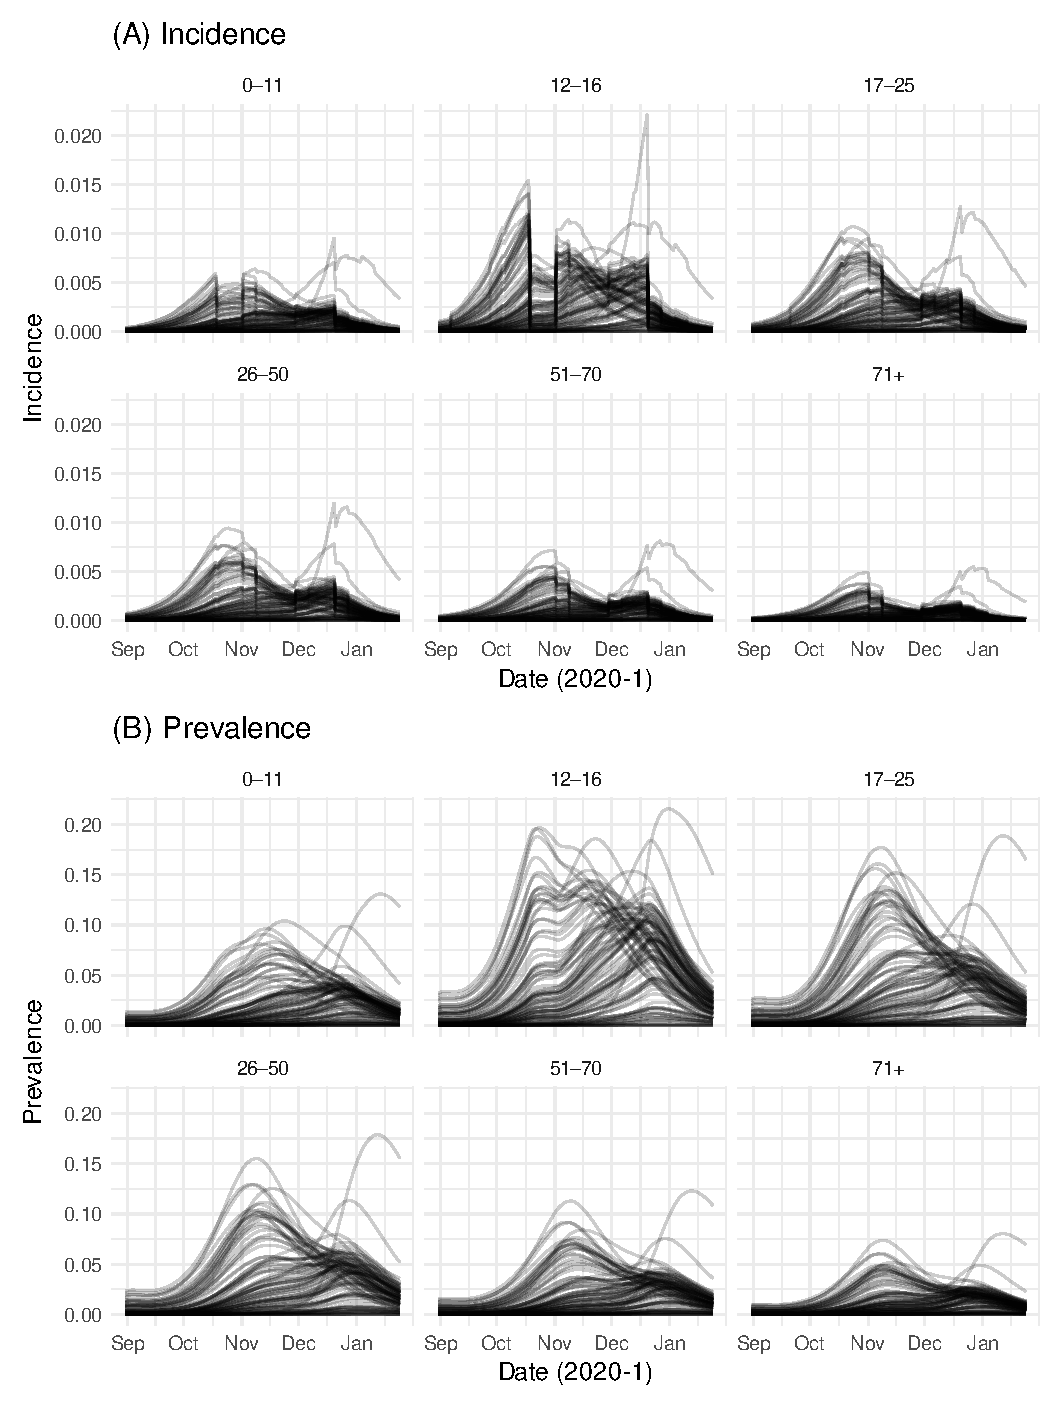
\includegraphics[width=.9\paperwidth]{SEIR/sim/data}}
    \caption[Simulated data]{%
        Incidence (top) and prevalence (bottom) for the 100 simulated data sets as a proportion of each stratum.
        Prevalence shown is $\bar{p}_{kat}$, the true population prevalence on each day, excluding sampling noise.
        Each line represents one simulation.
    }
    \label{SEIR:fig:sim-data}
\end{figure}

% Furthermore, the combination of the posteriors across all simulations should recover the prior.

To check the performance of the inference procedure, I calculated the coverage of the 50\%, 75\%, and 95\% central credible intervals for each parameter and simulation.
I define coverage as the proportion of simulations where the true value of the parameter in that simulation was within the credible interval.
This procedure is a simplified version of simulation-based calibration~\autocites{cookValidation}{taltsValidating}.
The coverage for each parameter should equal the nominal probability (\eg the coverage should be 50\% for the 50\% credible intervals).
I constructed a confidence interval for the coverage using the Pearson-Klopper method implemented in the binom package~\autocite{binom1-1}.

The majority of the confidence intervals contain the nominal probability (see \cref{SEIR:fig:sim-coverage}).
There is a tendency for the coverage to be slightly lower than the nominal probability, suggesting that the credible intervals are slightly too narrow; this is a common problem when using random-walk MCMC.
\todo{cite issues with random-walk MCMC exploring space}
This is similar when considering coverage of the derived quantities incidence and prevalence (see \cref{SEIR:fig:sim-inc-prev}).
\begin{figure}
    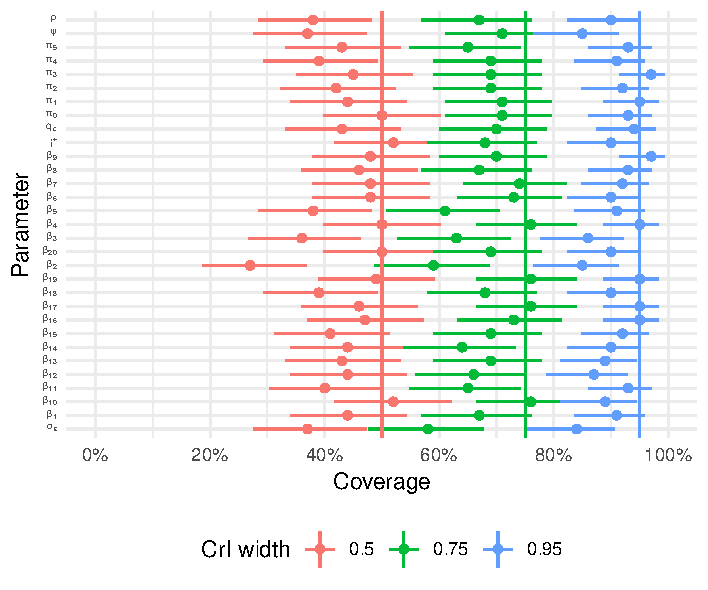
\includegraphics{SEIR/sim/coverage}
    \caption[Coverage of simulation study]{%
        Point estimate and 95\% confidence interval for coverage of the 50\%, 75\%, and 95\% central credible intervals for each parameter; see text for full definition.
        Vertical lines show the nominal coverage.
    }
    \label{SEIR:fig:sim-coverage}
\end{figure}
\begin{figure}
    \thisfloatpagestyle{empty}
    \vspace{-3cm}
    \makebox[\textwidth][c]{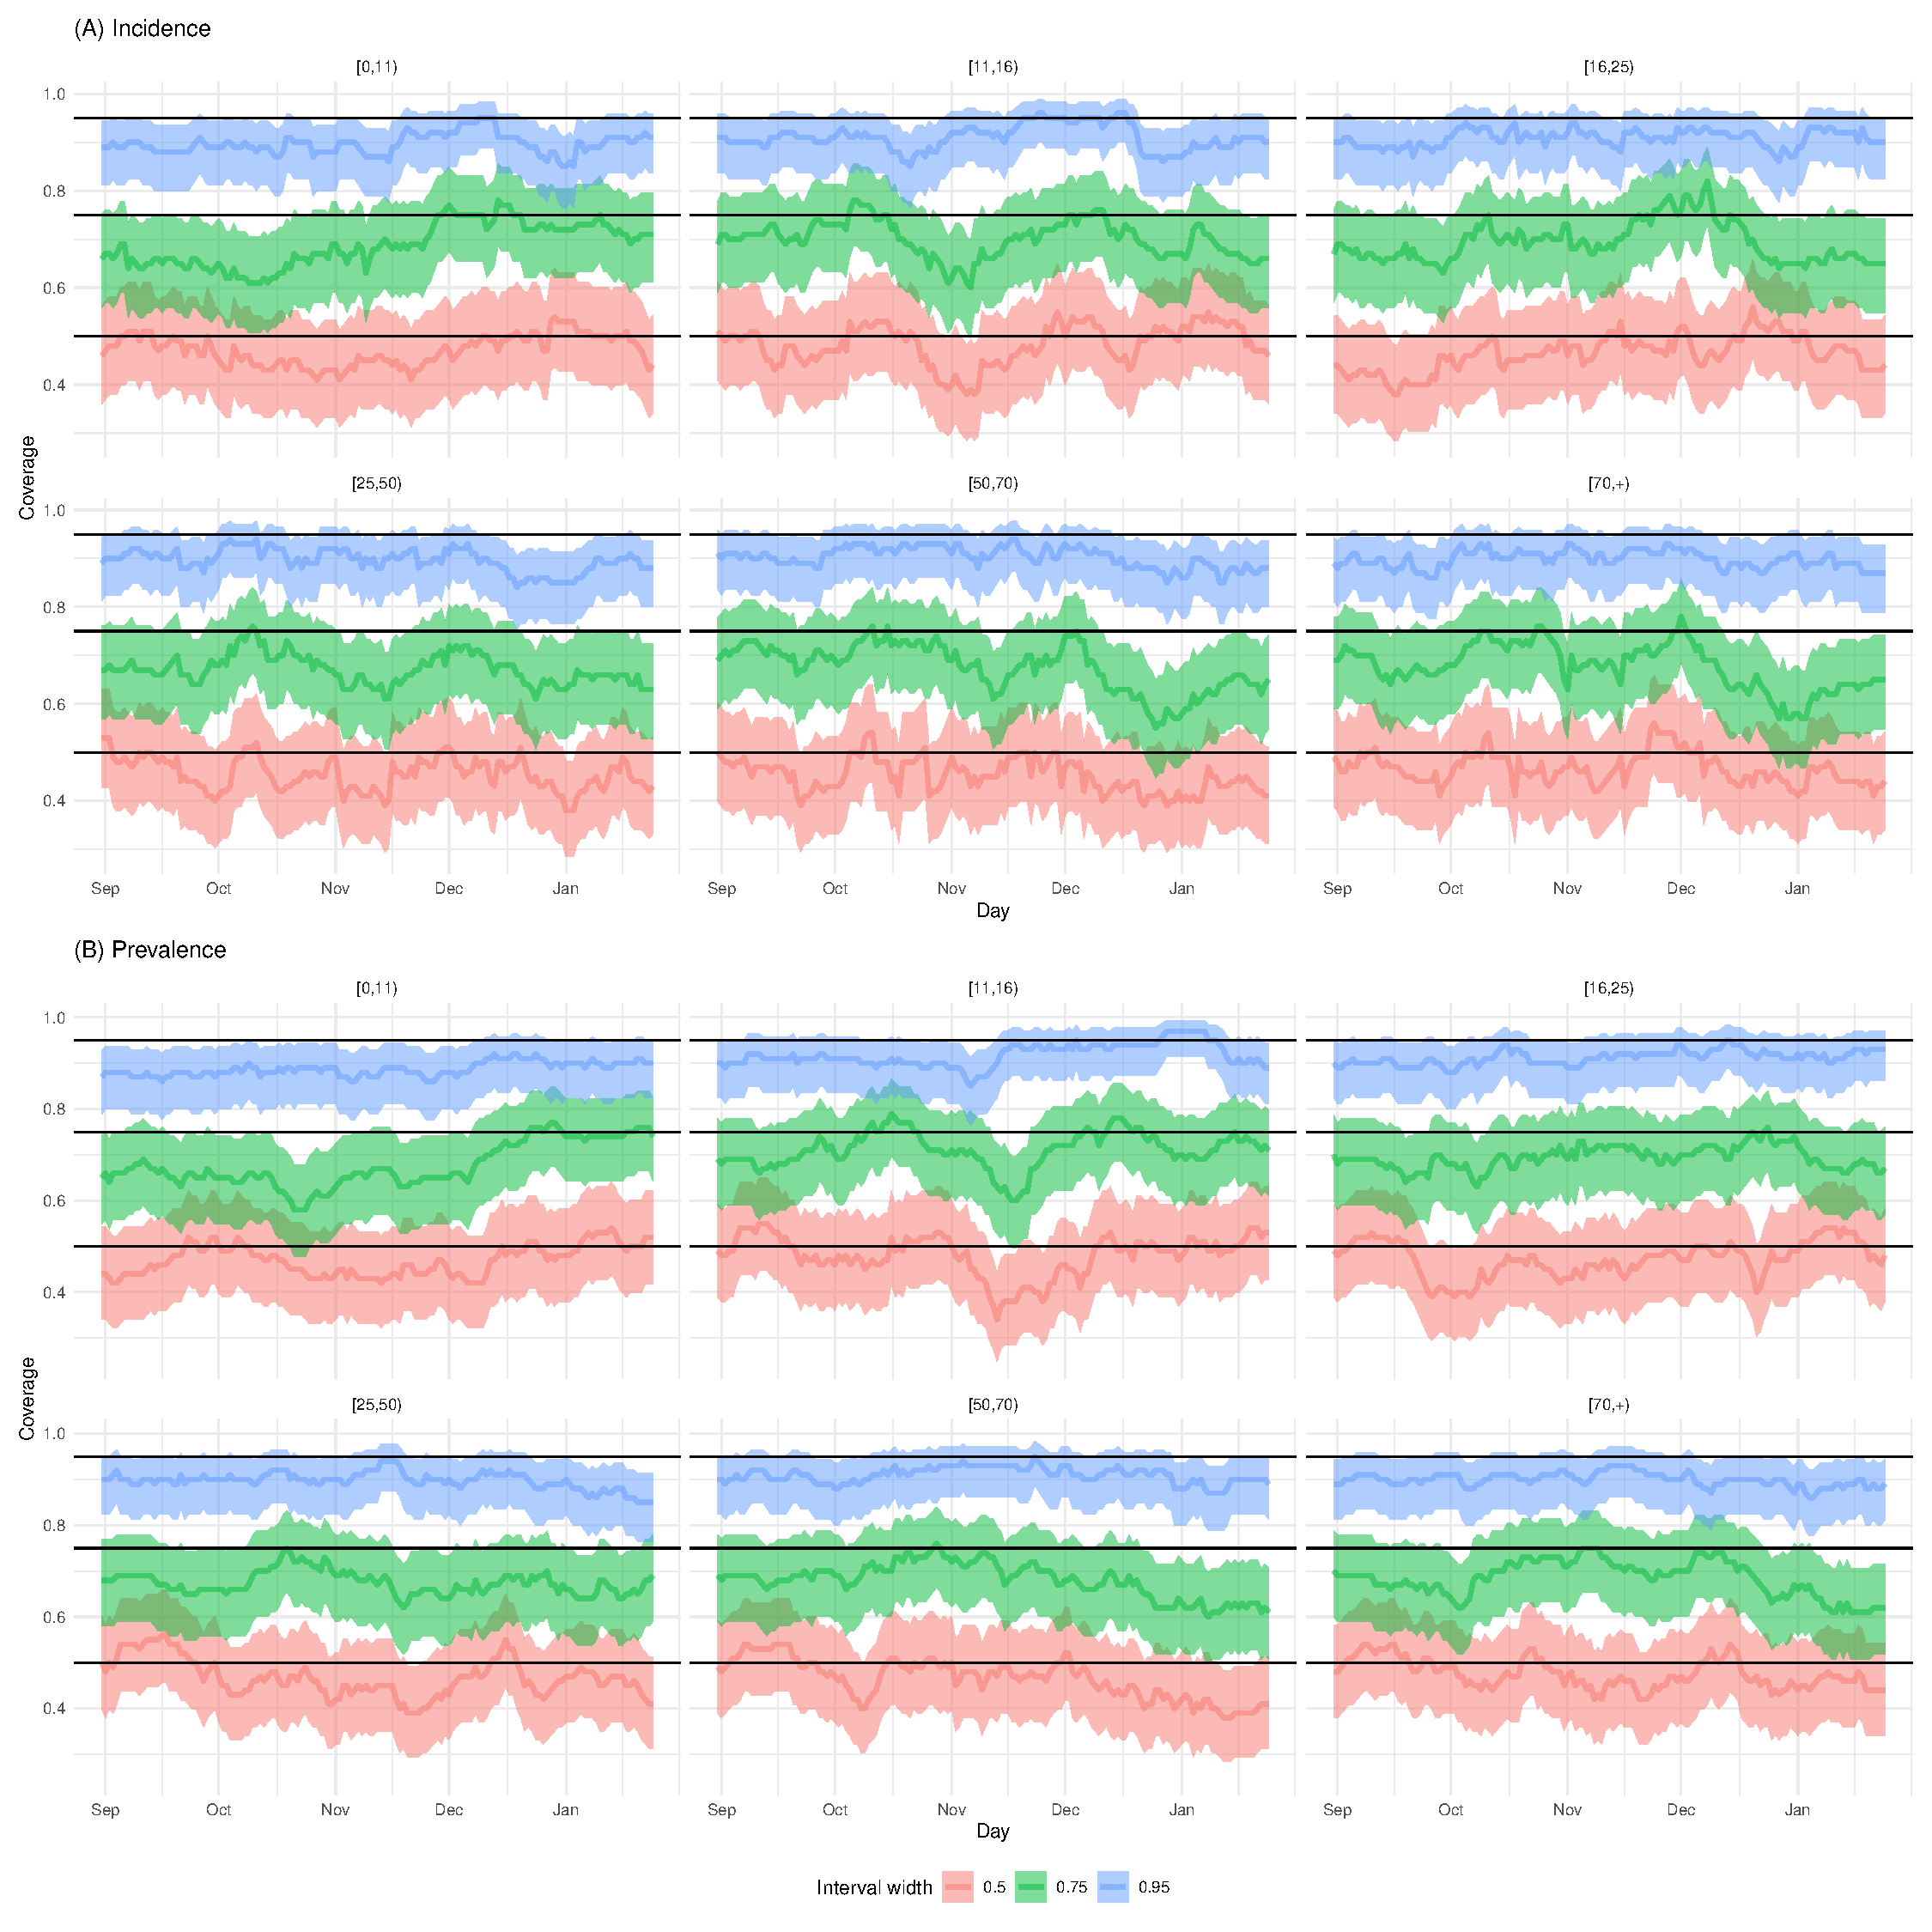
\includegraphics[width=0.9\paperwidth]{SEIR/sim/predictive_coverage}}
    \caption[Coverage of simulation study (derived quantities)]{%
        Point estimate and 95\% confidence interval for coverage of the 50\%, 75\%, and 95\% central credible intervals for incidence (top) and prevalence (bottom); see text for full definition.
        Horizontal lines show the nominal coverage.
    }
    \label{SEIR:fig:sim-inc-prev}
\end{figure}

In this setup, the parameters $i^+$, $q_c$, and $\psi$ are fully recovered; the other parameters are only partially so: their posterior has moved away from the prior but is still regularised by it (see \cref{SEIR:fig:true-vs-posterior}).
The ability to identify $q_c$ is an advantage of using data which includes measurements on children, unlike data on hospitalisations or deaths.
This suggests that these parameters are not practically identifiable in this setting.
The posteriors align very closely with the priors (not shown) which reinforces this finding.
The lack of identifiability for $\vec{\pi}$ aligns with previous work showing this parameter is structurally unidentifiable, \ie not identifiable even in the limit of infinite data~\autocite{dankwaStructural}.
\begin{figure}
    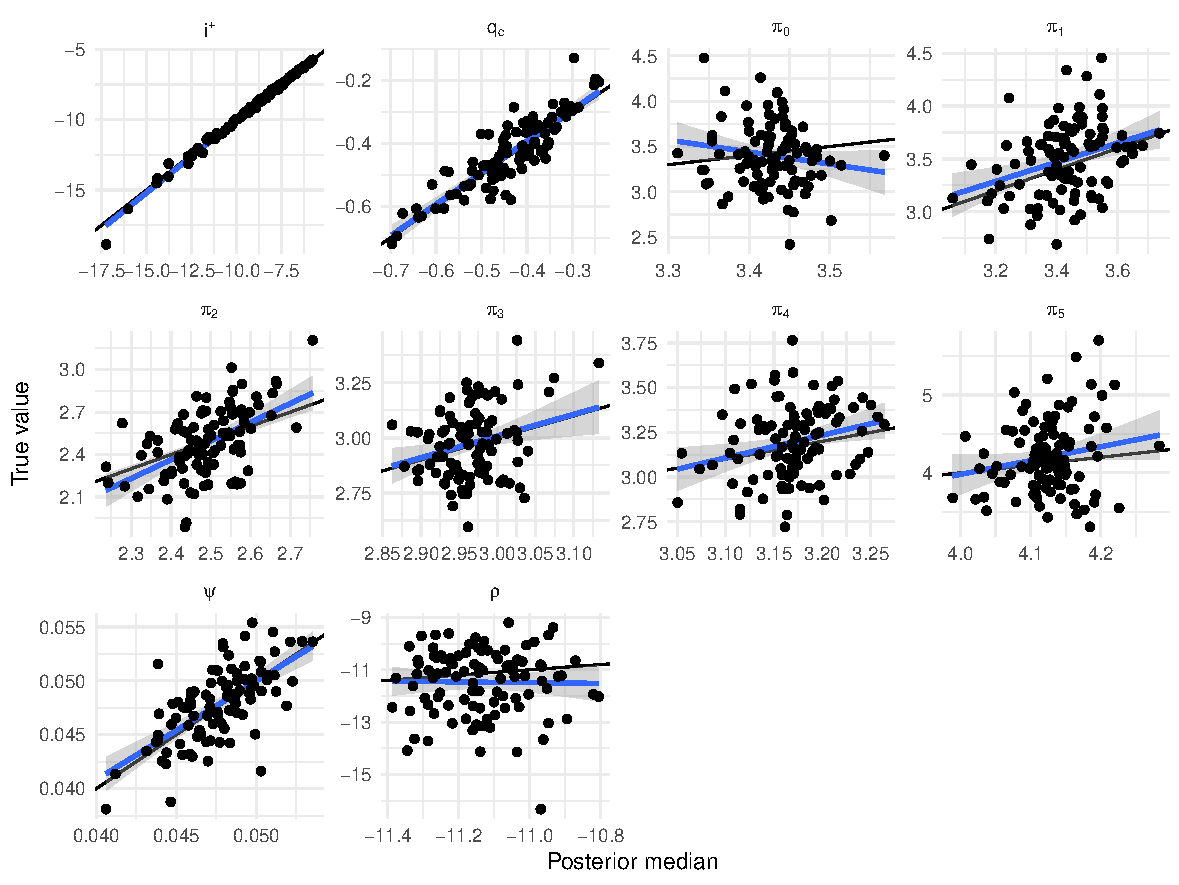
\includegraphics{SEIR/sim/true_vs_posterior}
    \caption[True vs posterior parameter values]{%
        True vs posterior median parameter values for each parameter in each simulation.
        The black line shows the line $y = x$ which the dots would lie on if the parameter is fully recovered.
        The blue line is a linear regression line.
        For $i^+$, $q_c$, and $\psi$, the posterior recovers the true values.
        For $\vec{\pi}$ and $\rho$, the posterior median is very similar regardless of the true value.
    }
    \label{SEIR:fig:true-vs-posterior}
\end{figure}

\section{Application to CIS data} \label{SEIR:sec:application}

Overall the model fits the data well (see \cref{SEIR:fig:prev-young,SEIR:fig:prev-old}).
There are a few features of the data which are not captured by the model.
In particular, prevalence during October is higher in the 16--25s than the model predicts and lower in the 11--16s.
\begin{figure}
    \thisfloatpagestyle{empty}
    \vspace{-3cm}
    \makebox[\textwidth][c]{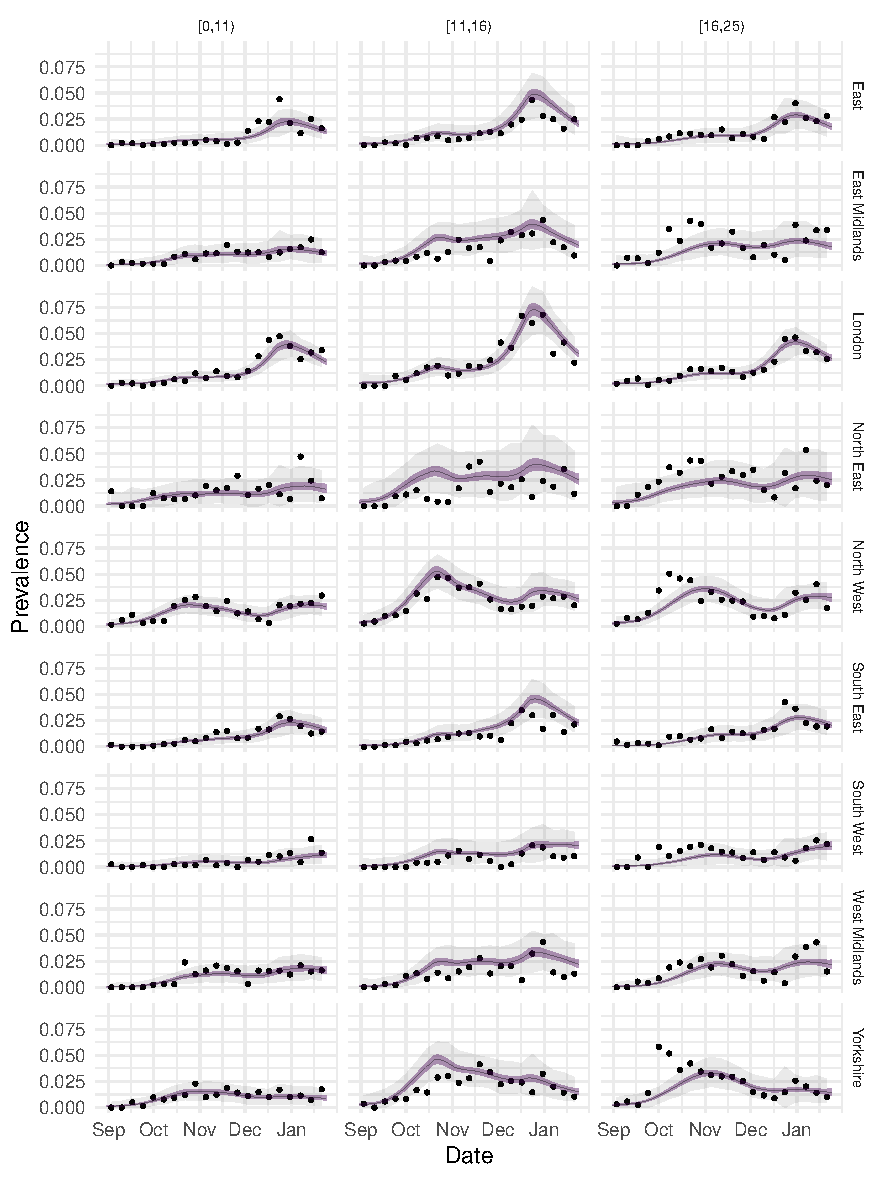
\includegraphics[width=.9\paperwidth]{SEIR/CIS/prev_young}}
    \captionsetup{width=0.8\paperwidth}
    \captionof{figure}[SEIR prevalence goodness-of-fit (younger ages)]{%
        Goodness-of-fit to prevalence data by region and age for the younger three age groups (see \cref{SEIR:fig:prev-old} for the others).
        The central ribbon and line shows the posterior median and 95\% CrI estimate for the proportion of the relevant strata PCR positive on each day.
        The lighter outer ribbon is the 95\% CrI including the noise due to the sampling (\ie observation process), aggregated by week.
        The dots show the observed prevalence in CIS, aggregated by week.
        For a well-calibrated model, 95\% of the dots would be within the outer ribbon.
    }
    \label{SEIR:fig:prev-young}
\end{figure}
\begin{figure}
    \thisfloatpagestyle{empty}
    \vspace{-3cm}
    \makebox[\textwidth][c]{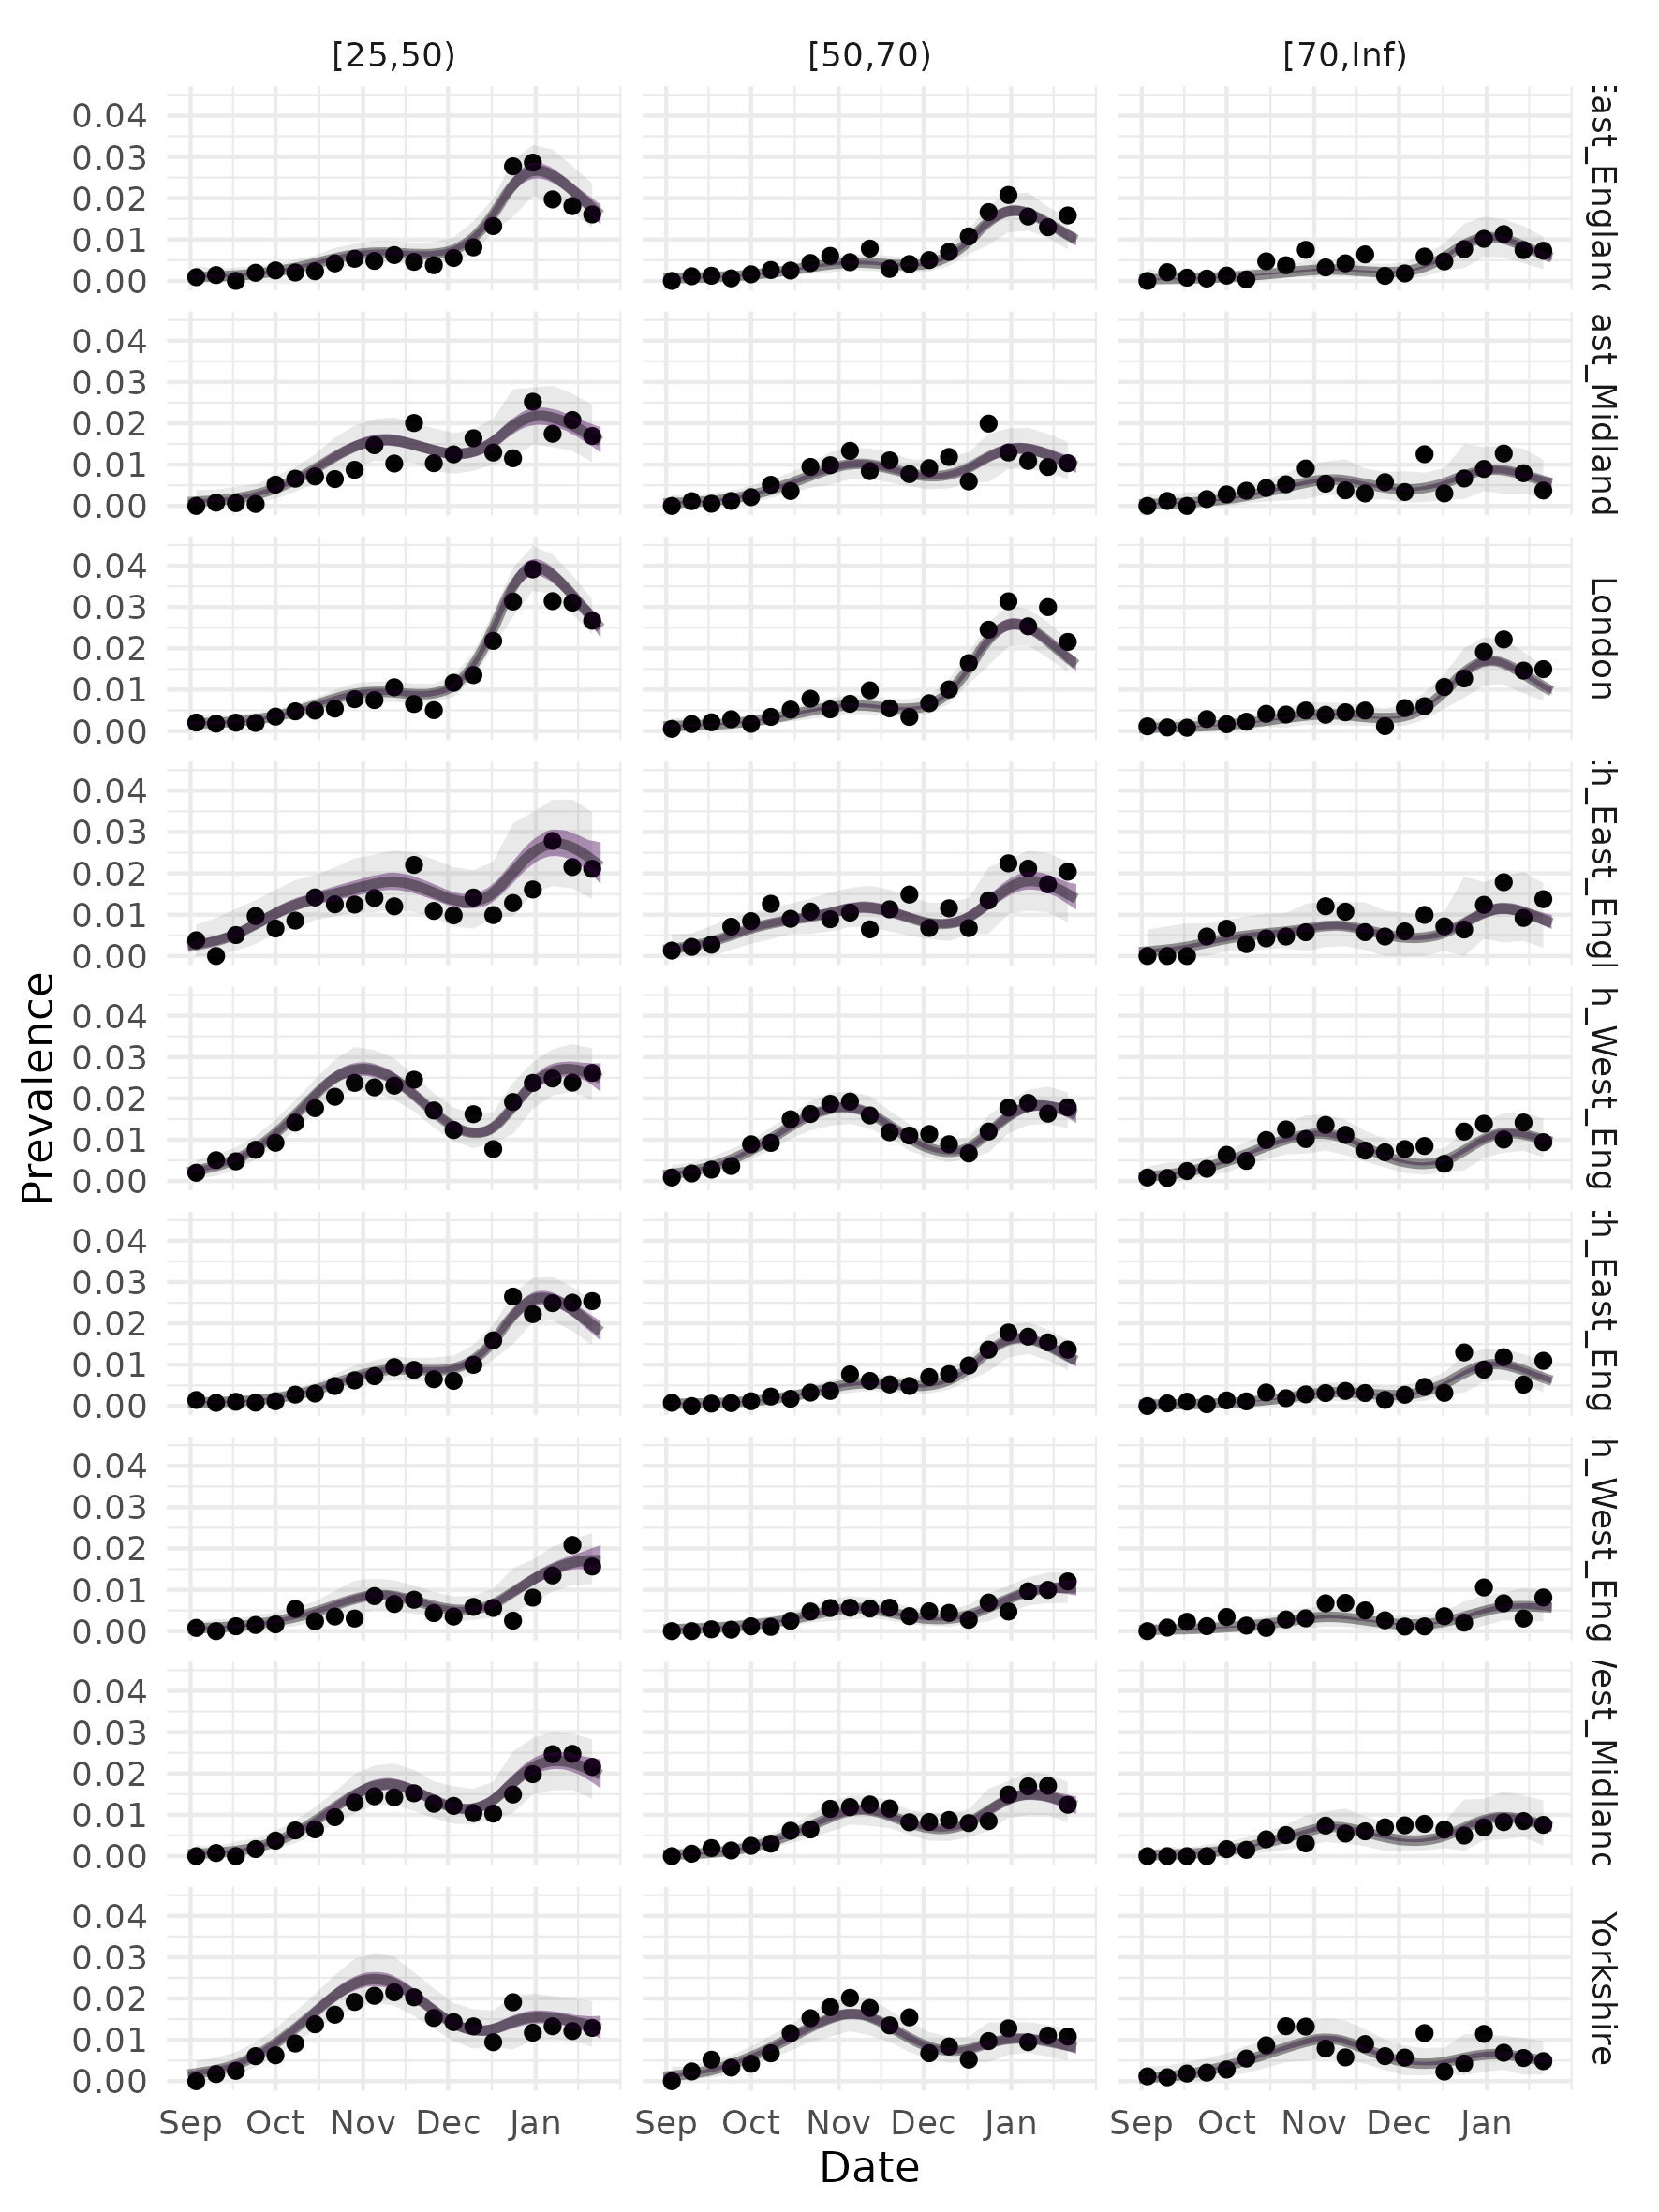
\includegraphics[width=.9\paperwidth]{SEIR/CIS/prev_old}}
    \captionsetup{width=0.8\paperwidth}
    \captionof{figure}[SEIR prevalence goodness-of-fit (older ages)]{%
        Goodness-of-fit prevalence for the older three age groups (see \cref{SEIR:fig:prev-young} for the other age groups and details).
    }
    \label{SEIR:fig:prev-old}
\end{figure}

The 11--16 age group (roughly corresponding to compulsory secondary school education) is estimated to have the highest incidence (see \cref{SEIR:fig:incidence}).
Incidence is smooth within each week but shows discontinuities between weeks.
This is because the parameters within $\matr{\beta}(t)$ are constant within each week.
A constant $\matr{\beta}(t)$ leads to exponential growth over short time periods, once the initial dynamics have died out.
When the peak in incidence is estimated to occur varied by region, but due to this reason, is almost always on a Sunday (see \cref{SEIR:fig:peak-incidence}).
For Yorkshire, the peak is estimated to occur in late October.
For all other regions, it is estimated to occur in late December or Early January, the period during which severe social distancing measures were applied.
\begin{figure}
    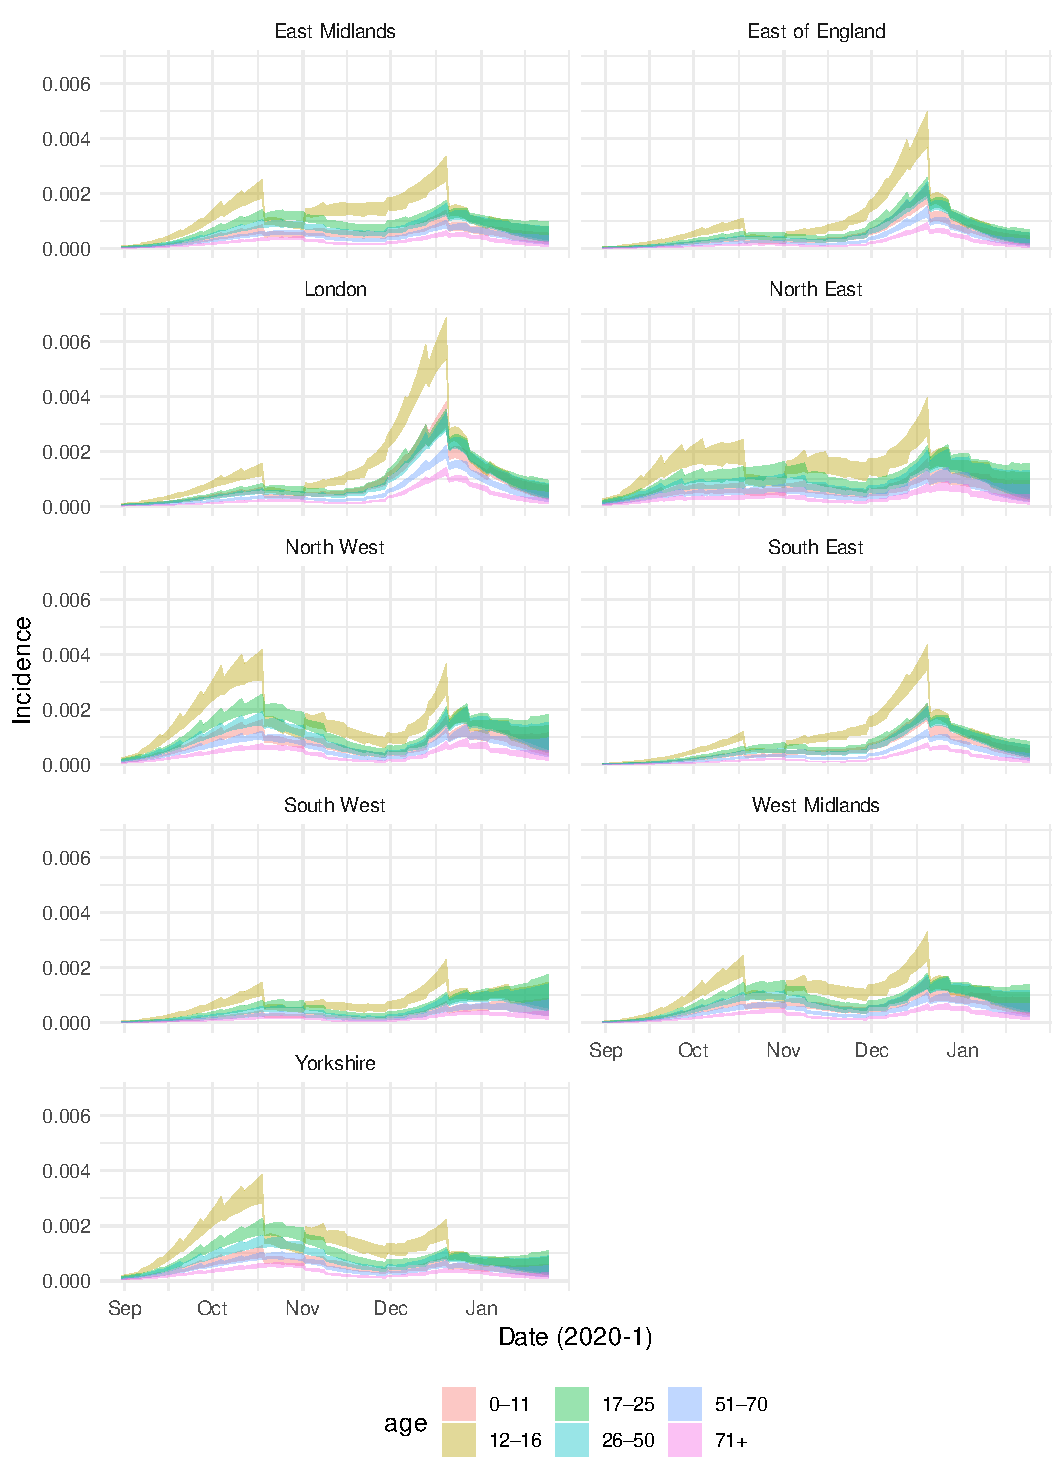
\includegraphics{SEIR/CIS/incidence}
    \caption[Posterior estimates of incidence]{%
        Posterior estimates (95\% CrI) of incidence by region and age.
        See main text for discussion.
    }
    \label{SEIR:fig:incidence}
\end{figure}

% \begin{figure}
%     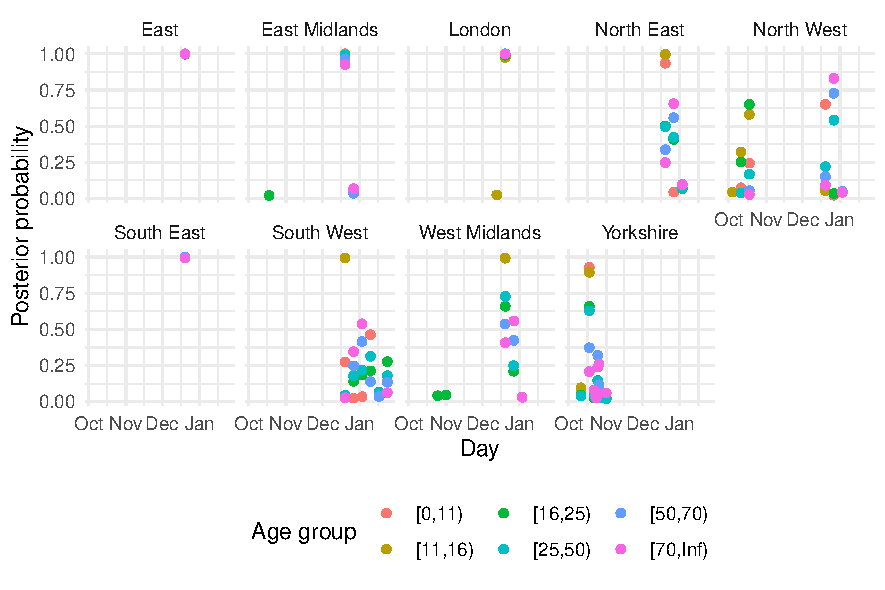
\includegraphics{SEIR/CIS/p_peak}
%     \caption[Posterior estimates of peak incidence timing]{%
%         Posterior probability of the peak incidence for each region and age combination occurring on each day.
%     }
%     \label{SEIR:fig:peak-incidence}
% \end{figure}


The parameters $\beta_t$ absorb all the time-varying changes in transmission not captured by Google mobility and school attendance data.
They trend downwards up until early December when they start increasing again.
Each region is estimated independently, however correlation is clear across the regions.

\begin{figure}
    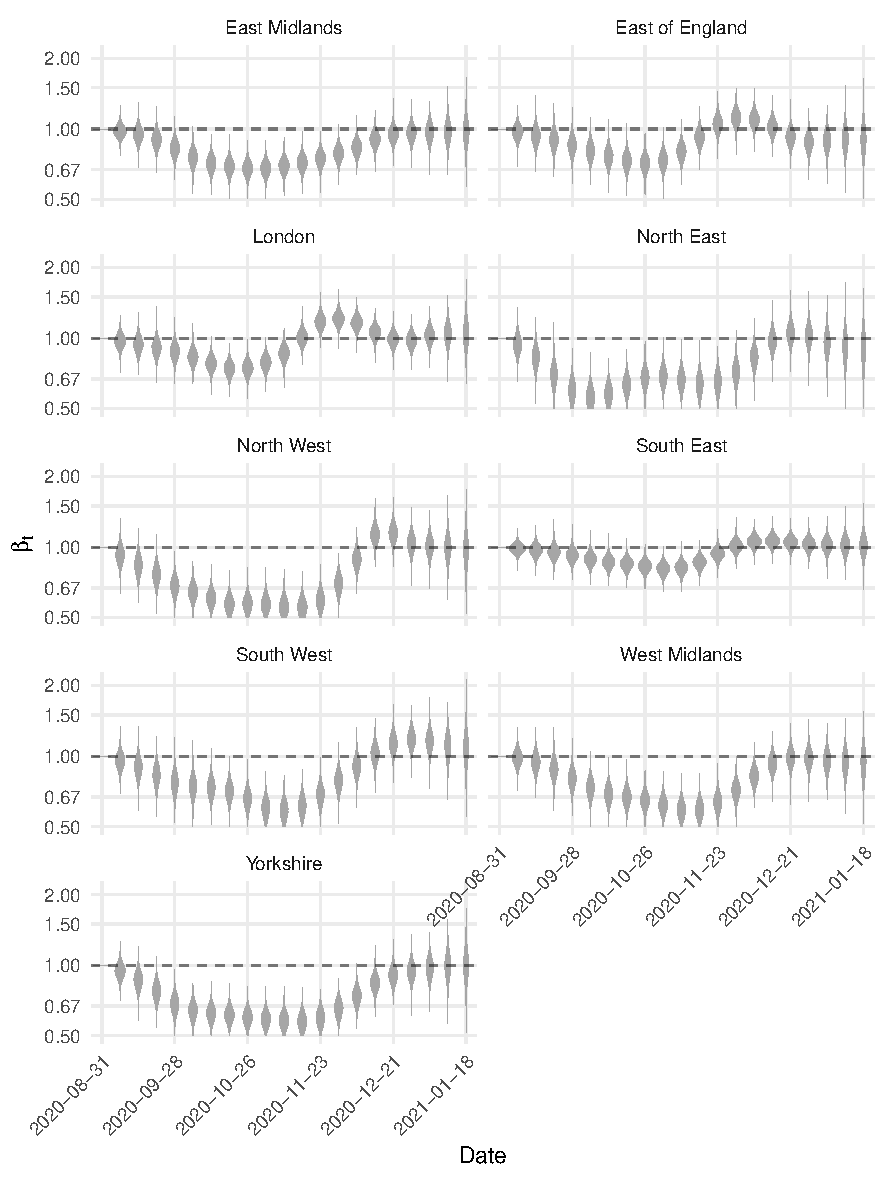
\includegraphics{SEIR/CIS/beta_walk}
    \caption[Posterior estimates of $\beta_t$]{%
        Posterior estimates $\beta_t$ for each week.
        Shown are ``violins'' where the width is proportional to the kernel-density estimated posterior density at that point.
        Values trend downwards until early December when an increase starts.
    }
    \label{SEIR:fig:beta-walk}
\end{figure}

One MCMC chain for the North West region appeared to get stuck, with very few moves after the first 100,000 iterations.
I reran this chain with a new seed.
Following this, all regions' MCMC chains converged, assessed using the Rhat statistic and ESS.
Rhat for all parameters is < 1.01, except $\sigma_\epsilon$ in London which had a Rhat of 1.018.
All parameters had ESS > 1000, except $\sigma_\epsilon$ in London and the East, which had ESS of 197 and 757 respectively.
As all the parameters of primary interest had high Rhat and ESS, and no parameters had large issues, the inference procedure is considered to have converged.

The \emph{attack rate} is the proportion of the population that have been infected at least once\todo{cite attack rate}.
In this model it is $1 - \vec{s}$.
The attack rate is highest in the $[11, 16)$ age group in the North West at 50\% (95\% CrI: 48\%--52\%) (see \cref{SEIR:fig:attack-rates}).
\begin{figure}
    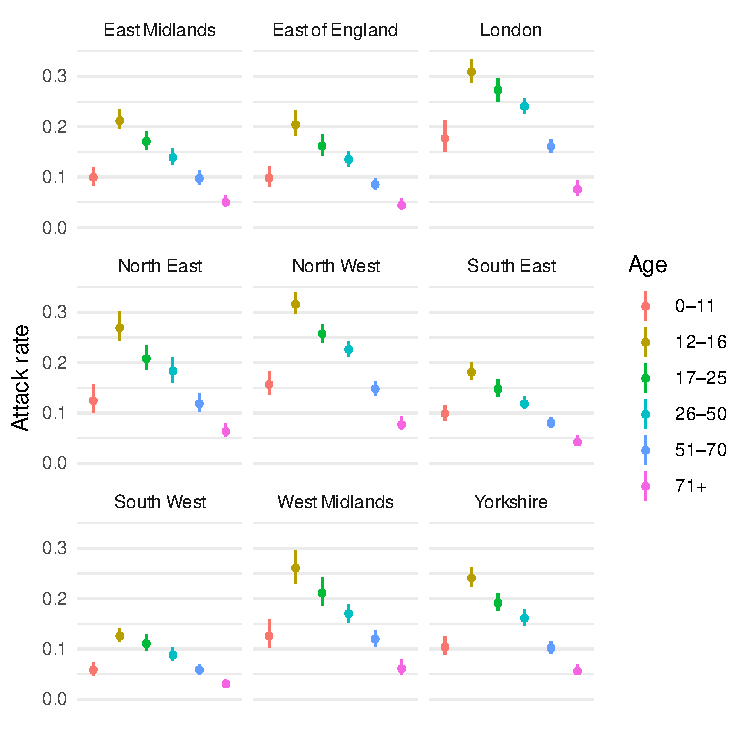
\includegraphics{SEIR/CIS/attack_rates}
    \caption{Posterior median and 95\% CrI of the attack rate in each region and age group.}
    \label{SEIR:fig:attack-rates}
\end{figure}

\todo[inline]{add comparison to backcalculation once I have those results}

\section{Discussion} \label{SEIR:sec:discussion}

The results in this chapter show the feasibility of fitting a mechanistic model using only data on prevalence.
If the distributions for length-of-stay in each compartment are known, then all other model parameters are able to be estimated.
This includes estimating the age distribution of the infections and the susceptibility of children.

Unlike most prior work, this modelling is based on a data source that is representative of the general population.
Therefore, the results are have fewer biases and informed by data to a greater extent than this work.
There is little-to-no ascertainment bias in the CIS, unlike sources relying on testing behaviour (in the UK, pillar 2 testing).
The CIS allows data-informed estimates of transmission in children, unlike sources relying on severe events that occur almost entirely in adults~\autocite{bhopalChildren}.

This approach provides additional understanding, compared to the approach in \cref{E-backcalc}.
For example, decomposing the change in transmission into changing contacts, $\matr{\kappa}(t)$, changing susceptibility $\vec{s}(t)$, and other unmeasured factors, $\beta(t)$.
By understanding which of these components is changing, policies can be better targeted.
If it is shown that $\beta(t)$ decreases, this implies that for a given amount of activity in the population, there is less transmission.
Such decreases might be beneficial as it allows society to operate in a more normal manner without increasing transmission.
Breaking the trade-off between transmission and activity is desirable because it reduces the disease burden without burdesome restrictions on individuals day-to-day lives.

The parameters $\beta_t$ absorb all the time-varying factors not captured by Google mobility and school attendance data.
Many factors contribute to the pattern in the $\beta_t$ values, which have a minima near the start of December.
While this analysis cannot establish causation, several hypotheses can be identified that are worth further investigation.
The decreases in $\beta_t$ over the autumn could be due to increased caution(\eg masking or stricter adherence to social distancing) and/or interventions short of a lockdown as cases and deaths increased~\autocite{jarvisEffect}, or the impact of local measures in the highest transmission areas~\autocite{scottCovid19}.
Local measures are not well captured by $\matr{\kappa}$ because the matrix was for the whole of England.
Allowing each region to have its own $\matr{\kappa}$ may capture the effect of local measures more accurately.
The increases in $\beta_t$ in December coincide with the rise of the Alpha variant~\autocite{lythgoeLineage}, known to be more transmissible~\autocite{daviesEstimated}.
A multiple variant model might be able to capture this rise more accurately.
Such a model would stratify positive tests in the CIS by pre-Alpha or Alpha variant.
Then, each variant would be explicitly included in the model to fit to this data.

These factors are correlated across the country.
This can explain that similar patterns emerge for $\beta_t$ in different regions (see \cref{SEIR:fig:beta-walk}), despite these being estimated independently (\ie there is no model structure which favours correlated values).
These correlations could be exploited to improve the precision of estimates with a more complex model which borrows information across regions.

The current model could be more flexible with regards to the age distribution of infections.
This would better exploit one of the strengths of the CIS: that there is data on all age groups.
In some regions, there appears to be a trade-off between the 11--16s and 16--25s, with the model misfitting in opposite directions (see \cref{SEIR:fig:prev-young}).
This implies that the data would allow identification of a more flexible age-based model.
Currently, the age distribution of infections is determined by $\matr{\beta}$, and to a lesser extent $\vec{\pi}$, the former of which only contains one inferred parameter that affects the age distribution, $\beta_c$.
More parameters could capture the age distribution more accurately.
There are various ways to increase the model's flexibility, including introducing additional susceptibility or infectiousness parameters, or by allowing these parameters to vary over time.
It is plausible that these distributions changed over time in a way not captured by $\matr{\kappa}$, for example due to the introduction and relaxation of control measures within schools.
$\matr{\kappa}$ only captures changes in in-school transmission through changes in school attendance, not incorporating the probability of transmission, which could be modelled as changes in $q_{aa}$ for $a$ of school age.
Similarly, there is evidence that $q_c$ is different for Alpha and pre-Alpha variants~\autocite{zhuRole}, which could again motivate these changing over time.

The weekly patterns in incidence are another limitation of the current parameterisation.
The random walk and contact matrices both vary only on the weekly timescale.
A daily random walk could provide more flexibility here.
However, this would greatly increase the number of parameters.
An alternative would be a smoothly-varying function or an approximation of a random walk such as that proposed by \textcite{ghoshApproximate}.

This discussion makes clear that the results are limited by the number of parameters, currently limited by the inference algorithm.
The algorithm used here tends to struggle with a large number of parameters.
Alternative proposal schemes, such as updating the parameters in blocks\todo{cite what RTM does?}, could help, or a more advanced algorithm such as NUTS (used elsewhere in this thesis).

Extending the estimates here to the rest of the pandemic would clearly be of interest.
I chose the end of the modelling period to coincide with the vaccination rollout.
Vaccination dramatically affects the transmission dynamics by introducing some additional immunity into the population.
Mechanistic models require explicit representation of this immunity\todo{cite something about vaccination}.

\todo[inline]{discuss comparisons with the backcalculation}

\section{Conclusion}

\todo[inline]{write conclusion and add to discussion once comparison with backcalculation is made}

\ifSubfilesClassLoaded{
  \listoftodos
}{}

\end{document}